





% Template for PLoS
% Version 1.0 January 2009
%
% To compile to pdf, run:
% latex plos.template
% bibtex plos.template
% latex plos.template
% latex plos.template
% dvipdf plos.template

\documentclass[10pt]{article}

% amsmath package, useful for mathematical formulas
\usepackage{amsmath}
% amssymb package, useful for mathematical symbols
\usepackage{amssymb}

% graphicx package, useful for including eps and pdf graphics
% include graphics with the command \inputgraphics
\usepackage{graphicx}
\usepackage{lscape}

% cite package, to clean up citations in the main text. Do not remove.
\usepackage{cite}

\usepackage{color} 

% Use doublespacing - comment out for single spacing
\usepackage{setspace} 
\doublespacing


% Text layout
\topmargin 0cm
\oddsidemargin 0.5cm
\evensidemargin 0.5cm
\textwidth 16cm 
\textheight 21cm

% Bold the 'Figure #' in the caption and separate it with a period
% Captions will be left justified
\usepackage[labelfont=bf,labelsep=period,justification=raggedright]{caption}

%load my own packages (not PLoS template)
\usepackage{textcomp, fixltx2e}
\usepackage{fullpage, lscape}
%\usepackage{lineno}

% Use the PLoS provided bibtex style
\bibliographystyle{plos2009}

% Remove brackets from numbering in List of References
\makeatletter
\renewcommand{\@biblabel}[1]{\quad#1.}
\makeatother


% Leave date blank
\date{}

\pagestyle{myheadings}
%% ** EDIT HERE **


%% ** EDIT HERE **
%% PLEASE INCLUDE ALL MACROS BELOW

%% END MACROS SECTION

\usepackage{Sweave}
\begin{document}
\Sconcordance{concordance:ligpaper.tex:ligpaper.Rnw:%
1}
\Sconcordance{concordance:ligpaper.tex:./rscripts.Rnw:ofs 1:%
18 1 42 1 13 1 6}
\Sconcordance{concordance:ligpaper.tex:ligpaper.Rnw:ofs 5:%
3 70 1 1 0 144 1}
\Sconcordance{concordance:ligpaper.tex:./fig_enz.Rnw:ofs 221:%
68}
\Sconcordance{concordance:ligpaper.tex:ligpaper.Rnw:ofs 222:%
219 9 1}
\Sconcordance{concordance:ligpaper.tex:./fig_mb2.Rnw:ofs 232:%
142}
\Sconcordance{concordance:ligpaper.tex:ligpaper.Rnw:ofs 233:%
230 12 1}
\Sconcordance{concordance:ligpaper.tex:./metaprot2.Rnw:ofs 246:%
56}
\Sconcordance{concordance:ligpaper.tex:ligpaper.Rnw:ofs 247:%
244 10 1}
\Sconcordance{concordance:ligpaper.tex:./fig_f2b.Rnw:ofs 258:%
186}
\Sconcordance{concordance:ligpaper.tex:ligpaper.Rnw:ofs 259:%
256 10 1}
\Sconcordance{concordance:ligpaper.tex:./fig_lci.Rnw:ofs 270:%
32}
\Sconcordance{concordance:ligpaper.tex:ligpaper.Rnw:ofs 271:%
268 11 1}
\Sconcordance{concordance:ligpaper.tex:./fig_degr.Rnw:ofs 283:%
83}
\Sconcordance{concordance:ligpaper.tex:ligpaper.Rnw:ofs 284:%
281 10 1}
\Sconcordance{concordance:ligpaper.tex:./fig_graphcorr.Rnw:ofs 295:%
111}
\Sconcordance{concordance:ligpaper.tex:ligpaper.Rnw:ofs 296:%
293 10 1}
\Sconcordance{concordance:ligpaper.tex:./fig_graphcorr2.Rnw:ofs 307:%
171}
\Sconcordance{concordance:ligpaper.tex:ligpaper.Rnw:ofs 308:%
305 14 1}
\Sconcordance{concordance:ligpaper.tex:./metaprot_plot.Rnw:ofs 323:%
88}
\Sconcordance{concordance:ligpaper.tex:ligpaper.Rnw:ofs 324:%
321 19 1 1 17 31 0 1 2 4 1 1 45 42 0 1 2 3 1 1 34 42 0 1 2 3 1 1 8 55 0 %
1 2 4 1}
\Sconcordance{concordance:ligpaper.tex:./fig_Psequestr.Rnw:ofs 536:%
101}
\Sconcordance{concordance:ligpaper.tex:ligpaper.Rnw:ofs 537:%
468 13 1}
\Sconcordance{concordance:ligpaper.tex:./fig_pyrpca.Rnw:ofs 551:%
11}
\Sconcordance{concordance:ligpaper.tex:ligpaper.Rnw:ofs 552:%
483 9 1}


% Title must be 150 characters or less
\begin{flushleft}
{\Large
\textbf{Litter nutrient contents controls extend of lignin decomposition via decomposer community composition in Beech litter }
}
\\
% Insert Author names, affiliations and corresponding author email.
% Insert Author names, affiliations and corresponding author email.
Lukas Kohl$^{1}$, % $^{3,\ast}$
Wolfgang Wanek$^{1}$, 
Katharina Keiblinger$^{2,3}$, 
Sonja Leitner$^{1,3}$, 
Maria Mooshammer$^{1}$, 
Ieda H\"ammerle$^{1}$, 
Lucia Fuchslueger$^{1}$, 
J\"org Schnecker$^{1}$, 
Thomas Schneider$^{4,5}$
Sandra Moll$^{7}$
Markus Gorfer$^{7}$
Joseph Strauss$^{7}$
Katharina Riedel$^{4,6}$
Leo Eberl$^{4,5}$
Sophie Zechmeister-Boltenstern$^{2,3}$, 
Andreas Richter$^{1}$,
\\
\bf{1} Department of Chemical Ecology and Ecosystem Research, University of Vienna, Althanstrasse 14, A-1090 Vienna, Austria
\\
\bf{2} Federal Research and Training Centre for Forests, Natural Hazards and Landscape, Department of Soil Biology, Seckendorff-Gudent-Weg 8, A-1131 Vienna, Austria
\\
\bf{3} Current address: Institute for Soil Science, University of Natural Resources and Life Sciences, Peter Jordan-Stra\ss e 82, A-1180, Vienna, Austria
\\
\bf{4} Institute of Plant Biology, University of Zurich, Winterthurerstrasse 190, CH-8057, Zurich, Switzerland
\\
\bf{5} Current address: Institute of Plant Biology, University of Zurich, Zollikerstrasse 107, CH-8008, Zurich, Switzerland
\\
\bf{6} Current address: Institute of Microbiology, Ernst-Moritz-Arndt University of Greifswald, Friedrich-Ludwig-Jahn-Strasse 15, D-17487 Greifswald, Germany
\\
\bf{7} Current address: Department of Applied Genetics and Cell Biology, University of Natural Resources and Life Sciences, Muthga\ss e 18, A-1190, Vienna, Austria

$\ast$ E-mail: Corresponding author@institute.edu
\end{flushleft}

\newpage
% Please keep the abstract between 250 and 300 words
\section*{Abstract}

Lignin is a major component of plant litter and is considered highly resistant to decomposition. Polymeric carbohydrates, in contrast, are more easily accessible carbon sources. We studied the decomposition rates of these two compound classes, to which extent they are controlled by litter C:N:P stoichiometry, and whether this control changes over time. Therefore, we conducted a 15-months mesocosm experiment under controlled climatic conditions, comparing beech litter of different N and P contents, which was sterilized and re-inoculated with a litter/topsoil mixture from one of the sites to ensure identical microbial communities at the start of the experiment. Lignin and carbohydrate decomposition rates were calculated for 2 periods (0-6 months and 6-15 months) by pyrolysis-GC/MS.

Positive correlations of carbohydrate decomposition rates with litter N content were found during the entire experiment. Lignin decomposition rates during the initial period were highly variable and negatively correlated to litter P content and positively correlated to the microbial P demand (C:P\textsubscript{litter}/C:P\textsubscript{microbial}). During the later stage, both lignin and carbohydrate decomposition loss were positively correlated to N contents and respiration. Initial lignin decomposition rates were highest in litter with low fungi:bacteria ratios, which occurred in N and P poor litter.

Our results showed that a substantial amount of lignin can be degraded during early decomposition. In the present study, early lignin decomposition was coupled to low N and P availability, and the establishment of K-strategist microorganisms. However, early lignin decomposition rates did not depend on fungi, which are commonly assumed to mediate lignin decomposition, or stoichiometric conditions that favor fungal growth. 

%\linenumbers %not from the template: start line numbers here.
\newpage%not in original layout
\pagestyle{empty}
\section*{Introduction}

Plant litter is quantitatively dominated by macromolecular compounds. In foliar litter, lignin and carbohydrate polymers together make up 40-60\% of litter dry mass \cite{Berg2008}, while leachable substances ("DOM") account for only 1.5-6\% \cite{Don2005}. The breakdown of these high molecular weight compounds into smaller molecules accessible to microbes is mediated by extracellular enzymes and considered rate limiting for decomposition processes \cite{Sinsabaugh2010}

Litter decomposition models generally follow the concept that organic compounds in litter form up to three independent pools of increasing recalcitrance, i.e. (1) soluble compounds, (2) cellulose and hemi-celluloses, and (3) lignin and waxes (cutin and suberin). Soluble compounds are most accessible to microbes and are usually consumed first, followed by regular polymers, such as cellulose. Lignin is not degraded until accumulated to a certain, critical level when it inhibits the degradation of less recalcitrant compounds\cite{Berg1980, Couteaux1995, Moorhead2006, Adair2008}. These pools are usually quantified by gravimetric determination of the amount of cellulose, hemi-celluloses and lignins after sequential extractions with selective solvents. These methods were repeatedly criticized for being unspecific for lignin determination \cite{Hatfield2005}. When analyzed with alternative methods (NMR, CuO-oxidation, Pyrolysis-GC/MS), extracted lignin fractions were shown to contain also many other substances \cite{Preston1997}.

Recent studies based on more specific methods to determine litter lignin contents question the assumed intrinsic recalcitrance of lignin. Isotope labeling experiments with soils and litter/soil mixtures, undertaken both in-situ and under controlled conditions,  revealed mean residence times of lignin in soils are in the range of 10-50 years, much less then expected and shorter than that of bulk soil organic matter or many other carbon compounds \cite{Amelung2008, Thevenot2010a, Bol2009}. Also, the capability to degrade lignin was demonstrated for several bacterial taxa in addition to fungi \cite{Bugg2011}.

For leaf litter, lignin depletion even at early stages of decomposition and lignin decomposition rates that decreased during decomposition were recently reported by Klotzb\"{u}cher and colleagues \cite{Klotzbucher2011}. Based on these results, they proposed a new concept for lignin degradation in which fastest lignin degradation occurs during early litter decomposition when the availability of labile carbon sources is high. Lignin decomposition during late decomposition, in contrast, is limited by the availability of easily assimilated C and therefore slowes down. Additionally, the decomposition of lignin may also be dependent on the nutrient content of the litter and thus the status of the microbial community. During radical polymerization, significant amounts of cellulose and protein are incorporated into lignin structures \cite{Achyuthan2010}. In isolated lignin fractions from fresh beech litter, N contents twice as high as in bulk litter were found \cite{Dyckmans2002}. It was therefore argued that, while yielding little C and energy, lignin decomposition makes protein accessible to decomposers that is occluded in plant cell walls, and that lignin decomposition is therefore not driven by C but by the N demand of the microbial community ("Nitrogen mining theory", \cite{Craine2007}). 

In favor of the N mining theory, fertilization experiments indicated N exerts an important control on lignin degradation: N addition increased mass loss rates in low-lignin litter while slowing down decomposition in lignin-rich litter \cite{Knorr2005} and decreased the activity of lignolytic enzymes in forest soils \cite{Sinsabaugh2010}. Moreover, cellulose triggered a stronger priming effect in fertilized than in unfertilized soils indicating that the mineralization of recalcitrant carbon may be controlled by an interaction of N and labile C availability \cite{Fontaine2011}.

Addition of N has a different effect on litter decomposition than varying N levels in the litter \cite{Talbot2011}. This is due to the fact that leaf litter N is stored in protein and lignin structures and not directly available to microorganisms, while fertilizer N is added in the form of readily available inorganic N (ammonium, nitrate or urea). N-fertilization experiments can thus simulate increased N-deposition rates but not the effect of litter N on decomposition processes.

Our study therefore aimed at analyzing the effect of variations in beech litter nutrient (N and P) content and stoichiometry (C:N and N:P ratios) on lignin and carbohydrate decomposition rates. Towards this end, we followed the breakdown of lignin and polymeric carbohydrates by pyrolysis-GC/MS (pyr-GC/MS) during a mesocosm experiment under constant environmental conditions over a period of 15 month. In order to exclude effects resulting from different initial microbial communities, we sterilized beech litter samples from 4 different locations in Austria and re-inoculated them prior to the experiment with an litter/top-soil inoculum from one of the sites.  
[one sentence on metaproteome/qPCR here]

We addressed the following questions in our study:

(1) Is lignin decomposition delayed until late decomposition stages or are significant amounts of lignin already degraded during early litter decomposition, and if the timing of lignin decomposition depended on litter stoichiometry? We hypothesized, that ligin decomposition is initially slower in litter with a narrow C:N ratio (higher availability of assimilable nitrogen), than in litter with a high C:N ratio.

(2) Are high lignin degradation rates related to a higher fungal activity? We hypothesized that wider C:N and C:P ratios favor lignin degradation by fungi while narrow C:N and C:P ratios favor carbohydrate degradation by bacteria. 
% Results and Discussion can be combined.
\section*{Results}
\subsection*{Initial litter chemistry}
Initital litter chemistry (14 days after incubation) is presented in table \ref{initstoech}. C:N ratios between 41:1 and 58:1 and C:P ratios between 700:1 and 1300:1 were found, N:P ratios ranged between 15:1 and 30:1. No significant changes occurred during litter incubation except a slight decrease of the C:N ratio (41.8:1 to 37.4:1) found in the most active litter type (SW) after 15 month. Fe concentrations were more than twice as high for OS (approx. 450 ppm) than for other litter types (approx. 200 ppm). Litter Mn also was highly variable between litter types, ranging between 170 and 2130 ppm. Changes of micro-nutrient concentrations during litter incubation were significant, but in all cases \textless 15\% of the initial concentration. In initial litter, lignin accounted for 28.9-31.2\% and carbohydrates for 25.9-29.2\% of the total peak area of all pyrolysis products.

\subsection*{Mass loss, respiration and extractable organic carbon}

Litter mass loss was not significant after 2 weeks and 3 months, and significant for 2 litter types after 6 months. After 15 months, litter mass loss was significant for all litter types, ranged between 5 and 12 \% of the initial dry mass, and was strongly correlated to litter N content (R=0.794, p\textless 0.001). Detailed results were reported by \cite{Mooshammer2011}.

Highest respiration rates were measured at the first measurement after 14 days incubation (150-350 \textmu g CO$_2$-C d$^{-1}$ g$^{-1}$ litter-C), which dropped to 75 to 100 \textmu g CO$_2$-C d$^{-1}$ g$^{-1}$ litter-C after 3 months. After 6 and 15 months, respiration rates for AK and OS further decreased, while SW and KL showed a second maximum in respiration after 6 months days (fig \ref{fig:enz}). Accumulated respiration was correlated to litter mass loss (r=0.738, p\textless 0.001, n=20).%\footnote{or r=0.961, p=0.038, n=4 if means are compared are used.}

Soluble organic carbon concentrations decreased between the first three harvests (14 days to 6 months), and strongly increased to 15 months (from 0.1 to 0.7 mg C g$^{-1}$  d.w. to 1.5 to 4 mg C g$^{-1}$ d.w. after 15 months, fig. \ref{fig:enz}). After 14 days and 3 months, the highest soluble organic C concentration was found in SW litter followed by AK. Soluble organic C concentrations were weakly correlated with litter N content after 14 days (r=0.69, p\textless 0.001) and after 3 months (r = 0.65, p\textless 0.01), but were strictly correlated after 6 months (r=0.85, p\textless 0.001) and 15 months (r=0.90, p\textless 0.001).

%\begin{figure*}[t]
%\vspace*{2mm}
%\begin{center}
%\setkeys{Gin}{width=0.5\textwidth}
%<<doc, echo=F, results=hide, fig=T, height=7, width=7>>=
%timeseries(alldata$DOC/1000, alldata$days, alldata$Litter, pch=pch, pt.bg=colscale,  xlab="Incubation (days)", ylab="mg C g-1 d.w.", main="Extractable carbon", lwd=2)
%legend("bottomright", pt.bg=colscale, pch=pch, typlev, lty=1, lwd=2)
%@
%\end{center}
%\caption{Extractable organic carbon. Error bars indicate standard errors (n=5).}
%\label{fig:doc}
%\end{figure*}

\subsubsection*{Potential enzyme activities}
Potential extracellular enzyme activities were correlated with litter N, respiration and other decomposition processes (all R\textgreater 0.8, p\textless 0.001). Cellulase activity increased from first harvest onwards to 15 months, with a small depression after 6 months (Fig. \ref{fig:enz}), phenoloxidase and peroxidase activities reached their maximum after between 3 and 6 months (fig. \ref{fig:enz}). For all enzymes and at all time points, SW showed the highest and AK the lowest activity. Differences between these two sites were more pronounced in cellulase activity (SW 10x higher than AK) than in oxidative enzymes (4x higher). Conversely, the phenoloxidase/cellulase ratio was highest for AK and lowest for SW at all time points and decreased during litter decomposition. This indicates that microbial communities in AK litter invested more energy and nitrogen into degrading lignin and less into degrading carbohydrates than in litter from other sites. (fig. \ref{fig:enz}).

\subsubsection*{Microbial biomass abundance and community composition}
Microbial biomass contents ranged from 0.5 to 6 mg C g$^{-1}$ d.w., 0.05 to 5.5 mg N g$^{-1}$ d.w. and 0.05 to 3.5 mg P g$^{-1}$ litter d.w (fig. \ref{fig:mb}). In KL and OS microbial biomass buildup reached a plateau after 3 months, AK and SW showed further microbial biomass growth reaching a maximum of microbial C and N contents after 6 months (AK also for P). Microbial C:N ratios ranged between 6 and 18, C:P ratios between 8 and 35, and N:P ratios between 0.5 and 3.5 (fig. \ref{fig:mb}).

Litter microbial biomass was stoichiometrically homeostatic during the first 6 months (no or marginally negative correlations between microbial C:N:P and litter C:N:P, see also \cite{Mooshammer2011}), but after 15 months (microbial C:N:P ratios were significantly correlated to resource stoichiometry: R=0.53-0.64, all p\textless 0.002), when the homeostatic regulation coefficients \cite{Sterner2002} H\textsubscript{C:P}=1.68, H\textsubscript{C:N}=2.01, and H\textsubscript{N:P}=2.29 were found. Microbial C:N ratios were tightly constrained after 3 months (14.5 to 18.2) and 6 months (6.9 to 9.0), but significantly different between the two time points. Microbial C:P and N:P ratios were less constrained, with the highest variance between litter from different sites after 3 months incubation (fig. \ref{fig:mb}).

Fungi/bacteria ratios derived from metaproteomics data of the litter (one replicate per litter type and harvest) were highest after 14 days (5 to 12) and decreased during litter decomposition (1.7 to 3 after 15 months). The large differences in fungi/bacteria ratios between litter types decreased during decomposition. Fungal proteins were dominant in all litter types at all stages, but most prominent in SW and least pronounced in  AK. The fungi/bacteria ratios were negatively correlated to the ratios of lignin/cellulose decomposition and to LCI change during the first 6 months. In contrast, lignin decomposition rates were positively correlated with fungi/bacteria ratios after 15 months but not to the ratios of lignin/cellulose decomposition (fig. \ref{fig:f2b}). In addition, fungi: bacteria ratios were measured on a DNA basis (qPCR) the results showing a similar pattern between litter types and harvests but with a much larger fungal DNA dominance (ratios between 10-180). Fungi/bacteria ratios were highly correlated between protein- and DNA-based estimates (r=0.801, p\textless 0.001, with log-transformed qPCR ratios).

\subsection*{Pyrolysis-GC/MS and Lignin content}
In total 128 pyrolysis products were detected, quantified, identified and assigned to their origin (\ref{tab:phprod} -\ref{tab:nprod}). We found only minor changes in the relative concentration of litter pyrolysis products during decomposition, and differences between sites were small but well preserved during decomposition. However, the high precision and reproducibility of pyrolysis GC/MS analysis of litter allowed tracing small changes in lignin and carbohydrate abundance during decomposition. Lignin-derived compounds made up between 29 and 31 \% relative peak area (TIC) in initial litter, and increased by up to 3 \% over the first 6 months. Carbohydrate-derived pyrolysis products accounted for 26 to 29 \% in initial litter and decreased by up to 2.6 \% during litter decomposition. The pyrolysis-based LCI index  showed a small range between 0.517 and 0.533 initially (Fig. 4). During decomposition, LCI increased by up to 9 \% of the initial value, with SW showing the highest increase while in AK LCI decreased. The changes in LCI almost completely occurred over the first 6 months, with insignificant changes thereafter (fig. \ref{fig:lci}).

During the first 6 months of litter decomposition, between one and 6 \% of the initial lignin pool and between 4 and 17\% of the initial carbohydrate pool were degraded (Fig. \ref{fig:degr}). Lignin decomposition was highest in AK and KL litter, while KL, OS and SW decomposed carbohydrates fastest. Lignin preference values (\% lignin decomposed/\%carbohydrates decomposed) were lowest in SW and highest in AK litter (Figure 5). In AK litter, lignin macromolecules were 50 \% more likely to be decomposed than carbohydrates, while in SW litter carbohydrates were 10 times more likely to be decomposed (fig. \ref{fig:degr}). Between 6 and 15 months, no further accumulation of lignin occurred, lignin and carbohydrates were both degraded at the same rates and their relative concentrations remained constant (fig. \ref{fig:degr}).

\subsection*{Correlations between lignin and carbohydrate decomposition and litter chemistry, microbial community and decomposition processes}

Relationships between lignin and carbohydrate degradation, litter chemistry, microbial biomass and decomposition processes were tested after 6 and 15 months (tables \ref{corrtable} and \ref{corrtable2}) including data presented by \cite{Mooshammer2011} and \cite{Leitner2011}. After 6 months, we found that the ratio of lignin/cellulose degradation was positively correlated with the ratio of phenoloxidase/cellulase (R=0.599, p=0.005) and peroxidase/cellulase (R=0.734 p\textless 0.001, table \ref{corrtable}). Carbohydrate decomposition was positively correlated with litter N content, and negatively with litter C:N ratios and litter-microbial C:N imbalances. In contrast, lignin decomposition was negatively correlated to litter P, but positively with litter C:P and N:P ratios, and litter-microbial C:P and N:P imbalances (fig. \ref{fig:cor1}). After 15 months, the ratio of lignin/carbohydrate decomposition was not related to stoichiometry or elemental composition any more. Most interestingly, lignin and carbohydrate decomposition exhibited the same controls, being positively correlated to soluble organic C, litter N and litter P (table \ref{corrtable2}). Mass loss and accumulated respiration were positively correlated to lignin and carbohydrate decomposition (table \ref{corrtable2}), a pattern that we did not find for lignin decomposition in the early decomposition phase (table \ref{corrtable}).

\section*{Discussion}

We used beech litter collected at different sites to study the effect of litter quality on decomposition. Differences in litter quality led to different mass loss rates and the development of of different decomposer communities from the same inoculate. Lignin decomposition  was highly variable between litter of different quality within the first 6 month; lignin decomposition rates ranged from no detectable degradation (SW litter) to decomposition at bulk carbon loss rates (ie. no lignin accumulation, AK litter). Our results therefore provide further evidence that the use of extractive methods two measure lignin contents led to an underestimation of early lignin degradation rates, as recently suggested \cite{Klotzbucher2011}, and that substancial amounts of lignin can be degraded during early decomposition. In contrast, between 6 and 15 months, lignin was degraded at the same rate as bulk carbon in all litter, regardless of litter quality. During this time, the different lignin contents aquired within the first six months remained in place, but lignin contents no further increased.  

Our study was designed to investigate the effect of litter N and P contents on decomposition, and we chose our collection sites to provide litter with different N and P contents. We found positive correlations between litter N and bulk decomposition parametres like carbon mineralization rates and extracellular enzymatic activities, indicating litter decomposition was limited by litter N. No such correlation was found for litter P contents. However, AK litter, which had low contents in both N and P, had a lower C mineralization rate than KL and OS, which were had lower contents of N or P, respectively, than AK, suggesting a co-limitation of both elements. The use of litter of a single species from different sites minimized differences in other litter traits, and eg. initial carbohydrate and lignin contents of all samples fell in a narrow range for litter from all sites. However, litter N and P contents are also proxies for other litter traits not directly measurable (e.g. leaf morphology), which resulted from the plant’s response to nutrient availability (e.g. for low P adaptation see \cite{Vance2003}). N and P were also demostrated to be correlated to a wide area of leaf traits in plants (ref\footnote{good ref for leaf economy spectrum needed!}), and such leaf traits were successfully used to predict litter decomposeability in the past\cite{Cornelissen1997}. 

The composition of the microbial community changed with both by time (i.e. succession) and collection site (i.e. litter quality). While all samples measured were dominated by fungi, fungi:bacteria ratios decreased over time and were higher in nutrient-rich litter than in nutrient-poor litter (SW >> AK). Our results contradicted the often-cited predictions that higher N and P contents would favor bacterial over fungal growth because bacterial biomass has lower C:N and C:P ratios than fungal biomass \cite{Hodge2000}. In contrast, we found fungi : bacteria ratios were higher in nutrient-rich litter. Similar observations were reported by Güsewell and Gessner 2009, who suggested that bacteria compensate N deficiency by heterotrophic N fixation, and therefore colonize low-N litter more successfully. However, microbial decomposers excrete important amounts of N as extracellular enzymes, what further raise their N demand; a factor not represented in the biomass C:N ratios. The higher abundance of bacteria on low nutrient litter would also be explained if fungi produced more extracellular enzymes per biomass than bacteria, therefore have creating a more narrow C:N demand than bacteria even though their biomass has a wider C:N ratio. In result, bacteria-rich decomposers with more narrow C:N and C:P biomass develloped on low-nutrient sites, with more narrow C:N and C:P ratios, further increasing difference between microbial and litter stoichiometry. To consider both litter and microbial stoichiometry, we used C:X$_{litter}$ : C:X$_{consumer}$ ratios as integrated measure for nutrient availability to nutrient demand.



%Correlative analysis indicated a differential control over lignin and carbohydrate decomposition: Carbohydrate loss rates were coupled to bulk mineralization, while lignin decomposition during the later period (6-15 months) controlled by litter N contents (as are bulk litter and carbohydrate loss rates), lignin degradation rates during the first 6 months (and the extend of lignin accumulation over the whole decomposition process) were differentially regulated. 

% 

%We found a different trend during later decomposition (6 - 15 months), when contents of lignin and carbohydrates remained constant in all litter (ie. lignin and carbohydrates decomposed at bulk carbon loss rates) and litter quality affected bulk C mineralization rates, but did not lead to further shifts in the chemical composition of the litter.

%
Litter quality controlled the commposition of the microbial communities, and thereby the difference between litter and microbial stoichiometry, both of which were correlated to the extend of early lignin decomposition. Litter which accumulated more lignin had microbial communities with high fungi:bacteria ratios and lower differences between litter and microbial stoichiometry. Our results therefore indicate that lignin degradation is associated with bacteria-rich communities, a low availability of nutrients to decomposers, or both. 

Traditionally, the capability to completely degrade lignin was exclusively attributed to Basidomycota fungi \cite{Berg2008}. However, Basidomycota made up less than 5\% of fungal protein. Over the last years, the capeability to completely degrade lignin was demonstrated for several bacterial taxa (eg. actinomycetes, $\alpha$-, and $\gamma$-proteobacteria \cite{Bugg2011}). Of these three taxa, we found one ($\gamma$-proteobacteria) correlated to lignolytic activities after 3 and 6 months. The other two taxa (actinomycetes and $\alpha$-proteobacteria) were enriched after 15 months in all litter types, when lignin decomposition was found in litter from all sites (ie.  independent from litter quality). However, since our metaproteomic analysis only sporadically detected lignolytic enyzmes, we can not attribute lignolytic activities to specific taxa at this time. Nevertheless, our data indicates that corresponding trends for lignin degradation and fungal : bacterial protein abundance both along succession and between litter from different sites after 6 months (higher lignolytic activity at low fungi:bacteria ratios). Overall, lignin decomposition was not coupled to fungal abundance, hinting that bacterial contributions to lignin decomposition might be greater than traditionally assumed. Also, the activity of $\gamma$-proteobacteria deserves special attention in further studies on early litter decomposition. 

%Early lignin degradation increased with the difference between litter and microbial stoichiometry (both C:N$_{litter}$ : C:N$_{microbial}$ and C:P$_{litter}$ : C:P$_{microbial}$). These stoichiometric differences were higher for the bacteria-enriched lignin decomposing communities, due to both low-nutrient litter and nutrient-rich microbial biomass. Litter with early lignolytic activity was therefore characterized by different decomposer community compositions and a lower nutrient availability than non-lignolytic litter.and C:N$_{litter}$ : C:N$_{microbial}$

%However, a greater influence of P availability can be expected during early decomposition when nutrients are net-immobilized to cover the nutrient demand of an increasing microbial biomass \cite{Manzoni2010}. Also, more rapidly dividing microorganisms have a more narrow N:P demand than slow growing microorganisms (\cite{Keiblinger2010}), therefore the importance of P is higher during litter colonization.


Lignin degradation in the first 6 months was positively C:P$_{litter}$ : C:P$_{microbial}$ and C:N$_{litter}$ : C:N$_{microbial}$, ie. more lignin was degraded when the difference between litter and microbial stoichiometry was higher. Differentiating between the effects of these two stoichiometric ratios was difficult, since both were intercorrelated. Lignin decomposition rates were also negativly correlated to litter P, but not N contents and positively correlated to microbial biomass P contents, while carbohydrate decomposition was positively correlated to litter N. This would indicating a differential control of lignin (inhibited by P) and carbohydrate (stimulated by N) decomposition. Also, actively lignin degrading litter (AK and KL) net-mobilized insoluble litter P during this time, while in slowly lignin degrading litter (SW and OS) an accumulation of microbial P led to a decrease in soluble P. This suggests that lignin degradation increased the mobilisation of P from insoluble litter biomass into the rapidly recycled P fractions (biomass and disolved), and would explains higher lignin degradation rates in litter with high microbial P demand. However, such a nutrient mobilization by lignin degradation is commonly assumed for N, but not for P \cite{Craine2007}: Lignin (like humic compounds) does not provide sufficient C and energy to sustain the decomposers metabolism, but occludes important amounts of protein during polymerization \cite{Achyuthan2010}, which is available only after lignin degradation. Therefore, lignin degradation was proposed to constitute a strategy of N sequestration (N mining theory, \cite{Sinsabaugh2006, Craine2007}). 

The degradation of lignin and carbohyradate polymers depends on the excretion of different extracellular enzymes. Their production is N intensive, therefore a trade-off exists between the production of cellulolytic and lignolytic enyzmes \cite{Sinsabaugh2010}. Lignin decomposition was also suggested to allow decomposers direct competition by the early colonization of lignin rich sites \cite{Treseder 2011}. We found higher activities of both cellulolytic and lignolytic enzymes in N-rich litter, but their ratio was well correlated to lignin : carbohydrate decomposition. Lignin degradation yields less C and energy than carbohydrates degradation, but might provides additional N. When C:X$_{substrate}$ : C:X$_{consumer}$ is low, as it was the case for lignin degrading litter, additional carbon can not be used by decomposers to build up biomass. Therefore, the observed increase in lignolytic activities might result from a microbial strategy to optimize N allocation between cellulytic and lignolytic enzyme 
systems when additional C can not be untilized by the decomposer due to a lack of nutrients. 

%However, differences in initial lignin contents were marginal, and lignin degradation rate of sites with high lignin contents were lower than those of sites with low lignin contents. Lignin decomposition was therefore not triggered by elevated lignin contents that limit the use of other C sources as suggested by traditional models \cite{}. While Mn and Fe concentrations strongly varied between litter collected at different sites, however, concentrations were lowest in the litter with highest lignin decomposition rates (AK, see Table \ref{initstoech}), so Lignin decomposition rates were not limited by a lack of these these elements. Moreover, soluble organic C (“DOC”) was recently suggested to limit lignin decomposition since the process of lignin decomposition does not generate sufficient energy to power the metabolism of its decomposers (Klotzbücher 2011). However, we found highest (initial) DOC concentrations however were found in the two litter types that showed the highest and the lowest lignin decomposition rates (SW and AK). % a sentence of N & P fertilization vs. N & P variance in litter?


In summary, litter quality had profound influence on the litter decomposition process, including community decomposition and lignin accumulation. Lignin decomposition within the first six months was highly variable between litter of of the same species but differnet in nutrient contents, and ranged from no lignin degradation to lignin degradation at bulk litter C loss rates. It was associated with nutrient-rich microbial biomass on low-nutrient litter, ie. a high difference between litter and decomposer stoichiomtry, low fungi:bacteria ratios and an elevated abundance of $\gamma$-proteobacteria peptides. Differences in lignin contents aquired within the first six months remained in place during later decomposition, although - regardless of litter quality - lignin was not further accumulated between 6 and 15 months.

% You may title this section "Methods" or "Models". 
% "Models" is not a valid title for PLoS ONE authors. However, PLoS ONE
% authors may use "Analysis" 
% Do NOT remove this, even if you are not including acknowledgments
\section*{Material and methods}
\subsection*{Litter decomposition experiment}
Beech litter was collected at four different sites in Austria (Achenkirch (AK), Klausenleopoldsdorf (KL), Ossiach (OS), and Schottenwald (SW); referred to as litter types) in October 2008. Litter was cut to pieces of approximately 0.25cm\textsuperscript{2}, homogenized, sterilized twice by $\gamma$-radiation (35 kGy, 7 days between irradiations) and inoculated (1.5\% w/w) with a mixture of litter and soil to assure that all litter types share the same initial microbial community. From each type, four samples of litter were taken immediately after inoculation, dried and stored at room temperature. Batches of 60g litter (fresh weight) were incubated at 15 \textdegree C and 60\% relative water content in mesocosms for 15 months. For each litter type 5 replicates were removed and analyzed after 14, 97, 181 and 475 days. A detailed description of the litter decomposition experiment was published by \cite{Wanek2010}.

\subsection*{Bulk litter, extractable, and microbial biomass nutrient content}
To calculate litter mass loss, litter dry mass content was measurement in 5 g litter (fresh weight) after 48 h at 80  \textdegree C. Dried litter was ball-milled for further chemical analysis. Litter C and N content was determined using an elemental analyzer (Leco CN2000, Leco Corp., St. Joseph, MI, USA). Litter phosphorus content was measured with ICP-AES (Vista-Pro, Varian, Darmstadt, Germany) after acid digestion \cite{Kolmer}).
To determine dissolved organic C, dissolved N and P, 1.8 g litter (fresh weight) were extracted with 50 ml 0.5 M K\textsubscript{2}SO\textsubscript{4}. Samples were shaken on a reciprocal shaker with the extractant for 30 minutes, filtered through ash-free cellulose filters and frozen at -20 \textdegree C until analysis. To quantify microbial biomass C, N and P, further samples were additionally extracted under the same conditions after chloroform fumigation for 24 h  \cite{Brooks1985}. Microbial biomass was determined as the difference between fumigated and non-fumigated extractions . C and N concentration in extracts were determined with a TOC/TN analyzer (TOC-VCPH and TNM, Schimadzu), P was determined photometrically as inorganig P after persulfate digestion \cite{Schinner1996}.

Substrate to consumer stoichiometric imbalances \emph{C:X$_{imbal}$} were calculated as
\begin{equation}
 C:X_{imbal}=\frac{C:X_{litter}}{C:X_{microbial}} \label{eq:imbal}
\end{equation}
where \emph{X} stand for the element N or P.

\subsection*{Microbial Respiration}
Respiration was monitored weekly during the entire incubation in mesocosms removed after 6 month and on the last incubation day for all mesocosms using an infrared gas analyzer (IRGA, EGM4 with SRC1, PPSystems, USA). CO2 concentration was measured over 70 seconds and increase per second was calculated based on initial dry mass. Accumulated respiration after 6 month was calculated assuming linear transition between measurements, accumulated respiration after 15 month was estimated from respiration rates after 181 and 475 days.

\subsection*{Potential enzyme activities}

Potential activities of $\beta$-1,4-cellobiosidase (``cellulase''), phenoloxidase and peroxidase were measured immediately after sampling. 1 g of litter (fresh weight) was suspended in sodium acetate buffer (pH 5.5) and ultrasonicated. To determine cellulase activity, 200 \textmu l suspension were mixed with 25 nmol 4-methylumbelliferyl-$\beta$-D-cellobioside (dissolved in 50 \textmu l of the same buffer) in black microtiter plates and incubated for 140 min in the dark. The amount of methylumbelliferyl (MUF) set free in by the enzymatic reaction was measured flourimetrically (Tecan Infinite M200, exitation at 365 nm, detection at 450 nm). To measure phenoloxidase and peroxidase activity litter suspension was mixed 1:1 with a solution of L-3,4-dihydroxyphenylalanin (DOPA) to a final concentration of 10 mM. Samples were incubated in microtiter plates for 20h to determine phenoloxidase activity. For peroxidase activity, 1 nmol of $H_2O_2$ was added before incubation. Absortion at 450 nm was measured before and after incubation. All enzyme activities were measured in three analytical replicates. The assay is described in detail in \cite{Kaiser2010b}.

\subsection*{Pyrolysis-GC/MS}

Pyrolysis-GC/MS was performed with a Pyroprobe 5250 pyrolysis system (CDS Analytical) coupled to a Thermo Trace gas chromatograph and a DSQ II MS detector (both Thermo Scientific) equipped with a carbowax colomn (Supelcowax 10, Sigma-Aldrich). Between 2-300 \textmu g of dried and finely ground litter (MM2000 ball mill, Retsch) was heated to 600 \textdegree C for 10 seconds in a helium atmosphere. GC oven temperature was constant at 50 \textdegree C for 2 minutes, followed by an increase of 7 \textdegree C/min to a final temperature of 260 \textdegree C, which was held for 15 minutes. The MS detector was set for electron ionization at 70 eV in the scanning mode (m/z 20 to 300).

Peaks were assignment was based on NIST 05 MS library after comparison with measured reference materials. 128 peaks were identified and selected for integration either because of their abundance or diagnostic value. This included 28 lignin and 45 carbohydrate derived substances. The pyrolysis products used are stated in tables \ref{tab:phprod} -\ref{tab:nprod} For each peak between one and four dominant and specific mass fragments were selected, integrated and converted to TIC peak areas by multiplication with a MS response coefficient \cite{Schellekens2009, Kuder1998}. Peak areas are stated as \% of the sum of all integrated peaks.

A pyrolysis-based lignin to carbohydrate index ($LCI$) was calculated to derive a ratio between these two substance classes without influences of changes in the abundance of other compounds . 

\begin{equation}
 LCI=\frac{Lignin}{Lignin + Carbohydrates}
\end{equation}

Accounting for carbon loss, we estimate \% lignin and cellulose degraded during decomposition according to equation \ref{eq:closscorr}, where \emph{$\%_{init}$} and \emph{$\%_{act}$} stand for initial and actual \%TIC area of lignin or cellulose pyrolysis products, \emph{$C_{init}$} for the initial amount of C and \emph{$R_{acc}$} for the accumulated CO$_2$-C respired by a mesocosm.
\begin{equation}
 \%_{loss} = 100\cdot\frac{\%_{init}-\%_{act}}{\%_{init}}\cdot\frac{\left ( 1-R_{acc}\right ) }{C_{init}}
 \label{eq:closscorr}
\end{equation}

\subsection*{Metaproteome analysis and quantitative PCR}



From each harvest (14, 97, 181, and 475 days), one replicate per litter type was stored at -80\textdegree C for metaproteome analysis. 

For metaproteome analysis, 3 g of each sample were grounded in liquid nitrogen and extracted with Tris/KOH buffer (pH 7.0) containing 1\% SDS. Samples were sonicated for 2 min, boiled for 20 min and shaken at 4 \textdegree C for 1 h. Extracts were centrifuged twice to remove debris and concentrated by vacuum-centrifugation. An aliquot of the sample was applied to a 1D-SDS-PAGE and subjected to in-gel tryptic digestion. The resulting peptide mixtures were analyzed on a hybrid LTQ-Orbitrap MS (Thermo Fisher Scientific) as described earlier \cite{Schneider2010}. Protein database search against the UniRef 100 database, which also comprised the translated metagenome of the microbial community of a Mennesota farm silage soil \cite{Tringe2005} and known contaminants, was performed using the MASCOT Search Engine. A detailed description of the extraction procedure and search criteria was published by [2]. If more than one protein was identified based on the same set of spectra these  proteins were grouped together resulting in one protein cluster. The obtained protein/protein cluster hits were assigned to phylogenetic and functional groups and assignments were validated by the PROPHANE workflow (http://prophane.svn.sourceforge.net/viewvc/prophane/trunk/; \cite{Schneider2011}). Higher protein abundance is represented by a higher number of MS/MS spectra acquired from peptides of the respective protein. Thus, protein abundances were calculated based on the normalised spectral abundance factor (NSAF) \cite{Florens2006, Zybailov2006}. This number allows relative comparison of protein abundances over different samples \cite{Bantscheff2007}. 

Quantitative PCR was used to determine fungal and bacterial abundance as described recently \cite{Inselsbacher2010}. F:B ratios were calculated as the ratio between estimated amounts of bacterial and fungal DNA found.

\subsection*{Statistical analysis}
All statistical analyses were performed with the software and statistical computing environment R \cite{R}. If not mentioned otherwise, results were considered significant when p \textless 0.05. Due to frequent variance inhomogeneities Welch ANOVA and paired Welch's t-tests with Bonferroni corrected p limits were used. All correlations mentioned refer to Pearson correlations. [PCA/CCA] were calculated with the R package ``vegan'' \cite{vegan}.

\section*{Acknowledgments}
This study formed part of the national research network MICDIF (Linking microbial diversity and functions across scales and ecosystems, S-10007-B01, -B06 and -B07) by the Austrian Research Fund (FWF). Katharina Keiblinger is a recipient of a DOC-fFORTE fellowship of the Austrian Academy of Sciences. Vital support regarding Pyr-GC/MS measurments was given by Clemens Schwarzinger, Andreas Bl\"{o}chl and Birgit Wild.

%\section*{References}
% The bibtex filename
\bibliography{library}

\newpage
% \section*{Figure Legends}
% 
% \begin{figure}[!h]
% \begin{center}
% %\setkeys{Gin}{width=4in}
% %\setkeys{Gin}{width=\textwidth}
% %\SweaveInput{fig_enz}
% \end{center}
% \caption{
% {\bf Respiration rates, concentration of soluble organic C and potential extracellular enzyme activities} in decomposing beech leaf litter from a mesocosm experiment. Beech litter was collected in: triangles, Schottenwald (SW); diamonds, Ossiach (OS); squares, Klausenleopoldsdorf (KL); circles, Achenkirch, AK. Error bars indicate standard errors (n=5). Significant differences between litter types are presented by asterisks above the symbols, significant differences between time points by asterisks to the right of the curves. *, P\textless 0.05, **, P\textless 0.01, ***, P\textless 0.001, b.d. - below detection limit.}
% \label{fig:enz}
% \end{figure}
% 
% \begin{figure}[!h]
% \begin{center}
% %\setkeys{Gin}{width=4in}
% %\setkeys{Gin}{width=\textwidth}
% %\SweaveInput{fig_mb}
% \end{center}
% \caption{
% {\bf Microbial biomass C, N and P, microbial C:N:P stoichiometry and resource:consumer stoichiometric imbalance in these elements} in decomposing beech leaf litter from a mesocosm experiment. Beech litter was collected in: triangles, Schottenwald (SW); diamonds, Ossiach (OS); squares, Klausenleopoldsdorf (KL); circles, Achenkirch, AK. Error bars indicate standard errors (n=5). Significant differences between litter types are presented by asterisks above the symbols, significant differences between time points by asterisks to the right of the curves. *, P\textless 0.05, **, P\textless 0.01, ***, P\textless 0.001.}
% \label{fig:mb}
% \end{figure}
% 
% \begin{figure}[!h]
% \begin{center}
% %\setkeys{Gin}{width=4in}
% %\setkeys{Gin}{width=\textwidth}
% %\SweaveInput{fig_Psequestr.R}
% \end{center}
% \caption{
% {\bf Mobilization of litter P} (A) Insoluble litter P is mobilized into recycled P pools (dissolved and microbial biomass P) in lignin degrading litter (AK and KL), while the increase in biomass P on non lignin-degrading litter (OS and SW) origininates from soluble P. (B) correlation between mobilization of P and lignin accumulation, 0-6 months incubation. Beech litter was collected in: triangles, Schottenwald (SW); diamonds, Ossiach (OS); squares, Klausenleopoldsdorf (KL); circles, Achenkirch, AK. Error bars indicate standard errors (n=5).}
% \label{fig:phos}
% \end{figure}
% 
% 
% \begin{figure*}[h!]
% \vspace*{2mm}
% \begin{center}
% %\setkeys{Gin}{width=\textwidth}
% %\SweaveInput{metaprot2}
% \end{center}
% \caption{
% {\bf Protein abundance of fungal and bacterial taxa.} Litter was collected in Achenkirch (AK);, Klausenleopoldsdorf (KL); Ossiach (OS); Schottenwald (SW). Samples were analyzed after sterilization, re-innoculation and incubation for 14, 97, 181, or 475 days.}
% \label{fig:metaprot_barplot}
% \end{figure*}
% 
% 
% \begin{figure}[!h]
% \begin{center}
% %\setkeys{Gin}{width=0.7\textwidth}
% %\inputgraphics[width=4in]{figure_name.2.eps}
% %\SweaveInput{fig_f2b}
% \end{center}
% \caption{
% {\bf Fungi:Bacteria (F:B) ratios and their correlations with LCI change:} A: F:B protein abundance (left) and DNA (right) ratio. B: Correlations between F:B preotein abundance ratios and lignin loss (top), carbohydrate loss (mid) and lignin loss : carbon loss (bottom) for 0-6 months (left) and 6-15 months (right, errorbars indicate standard errors, n=4-5).  Beech litter was collected in: triangles, Schottenwald (SW); diamonds, Ossiach (OS); squares, Klausenleopoldsdorf (KL); circles, Achenkirch, AK. Error bars indicate standard errors (n=5). Significant differences between litter types are presented by asterisks above the symbols, significant differences between time points by asterisks to the right of the curves. *, P\textless 0.05, **, P\textless 0.01, ***, P\textless 0.001.}
% \label{fig:f2b}
% \end{figure}
% 
% \begin{figure}[!h]
% \begin{center}
% %\setkeys{Gin}{width=4in}
% %\setkeys{Gin}{width=\textwidth}
% %\SweaveInput{fig_lci}
% \end{center}
% \caption{
% {\bf Develoment of lignin to carbohydrate index (lignin : (lignin+carbohydrates), LCI)} during time of beech litter decomposition (left) or plotted against cumulative C loss (right). Errorbars indicate standard errors (n=4-5). The dashed line indicates a constant ratio between lignin and carbohydrates (i.e. no preferential decomposition of carbohydrates. Beech litter was collected in: triangles, Schottenwald (SW); diamonds, Ossiach (OS); squares, Klausenleopoldsdorf (KL); circles, Achenkirch, AK. Error bars indicate standard errors (n=5). Significant differences between litter types are presented by asterisks above the symbols, significant differences between time points by asterisks to the right of the curves. *, P\textless 0.05, **, P\textless 0.01, ***, P\textless 0.001.}
% \label{fig:lci}
% \end{figure}
% 
% \begin{figure*}[h!]
% \vspace*{2mm}
% \begin{center}
% %\setkeys{Gin}{width=\textwidth}
% %\SweaveInput{fig_degr}
% \end{center}
% \caption{
% {\bf Carbon loss corrected amounts of lignin and carbohydrates} degraded in beech litter collected in Achenkirch (AK), Klausenleopoldsdorf (KL), Ossiach (OS) and Schottenwald (SW). Carbon loss was calculated based on accumulated respiration for each mesocosm. Error bars indicate standard errors (n=4-5). The dashed line marks no discrimation during decomposition between lignin, carbohydrates and bulk carbon}
% \label{fig:degr}
% \end{figure*}
% 
% \begin{figure*}[h!]
% \vspace*{2mm}
% \begin{center}
% %\setkeys{Gin}{width=\textwidth}
% %\SweaveInput{fig_graphcorr}
% \end{center}
% \caption{
% {\bf Correlation between the LCI change or the ratio of lignin : carbohydrate decomposition ratio during the first 6 months of litter decomposition correlate to litter : microbe stoichiometric imbalances.} and change and Correlations between lignin accumulation during the first 6 month of litter incubation and stoichiometric resource:consumer imbalances. LCI is calculates as of lignin/(lignin+Carbohydrates).  Beech litter was collected in: triangles, Schottenwald (SW); diamonds, Ossiach (OS); squares, Klausenleopoldsdorf (KL); circles, Achenkirch, AK. *, P\textless 0.05, **, P\textless 0.01, ***, P\textless 0.001.}
% \label{fig:cor1}
% \end{figure*}
% 
% \begin{figure*}[h!]
% \vspace*{2mm}
% \begin{center}
% %\setkeys{Gin}{width=\textwidth}
% %\SweaveInput{metaprot}
% \end{center}
% \caption{
% {\bf Microbial commuity composition.} The first two components of a correspondance analysis (CA) of protein abundances found. Rectangles indicate samples of identical incubation time. Peptides were aggregated at class level (fungi and proteobacteria) or phylum level (other bacterial phyla): Dothideomycetes (Doth); Eurotiomycetes (Euro); Leotiomycetes (Leot); Saccharomycetes (Sacc); Sordariomycetes (Sord); Agaricomycetes (Agar); Tremellomycetes (Trem); Ustilaginomycetes (Usti); Thermotogae (Ther); Bacteroidetes (Bact); Actinobacteria (Acti); Cyanobacteria (Cyan); Firmicutes (Firm); Fusobacteria (Fuso); Verrucomicrobia (Verr); Dictyoglomi (Dict); Alphaproteobacteria (Alph); Betaproteobacteria (Beta); Gammaproteobacteria (Gamm); Deltaproteobacteria (Delt); Epsilonproteobacteria (Epsi). Taxa factor loadings were printed x2 for better readability. Correlations between CA 1, CA 2, and litter chemistry, microbial stoichiometry, and protein abundance of microbial taxa are stated in supplemental table \ref{catab}. 
% Arrows represent vectorial fittings of these variables calculated independently from the CA, plotted only if p\textless 0.05: Litter C content (C lit); C:X\textsubscript{Microbial}/C:X\textsubscript{Litter} (C:P imb, C:N imb).}
% \label{fig:metaprotpca}
% \end{figure*}
% 
% \newpage
% \begin{figure}[!ht]
% \begin{center}
% %\setkeys{Gin}{width=4in}
% \setkeys{Gin}{width=\textwidth}
% \SweaveInput{fig_enz}
% \end{center}
% %\caption{
% %{\bf Respiration rates, concentration of soluble organic C and potential extracellular enzyme activities} in decomposing beech leaf litter from a mesocosm experiment. Beech litter was collected in: triangles, Schottenwald (SW); diamonds, Ossiach (OS); squares, Klaus-nleopoldsdorf (KL); circles, Achenkirch, AK. Error bars indicate standard errors (n=5). Significant differences between litter types are presented by asterisks above the symbols, significant differences between time points by asterisks to the right of the curves. *, P\textless 0.05, **, P\textless 0.01, ***, P\textless 0.001, b.d. - below detection limit.}
% %\label{fig:enz}
% \end{figure}
% 
\begin{figure}[!ht]
\begin{center}
%\setkeys{Gin}{width=4in}
\setkeys{Gin}{width=\textwidth}
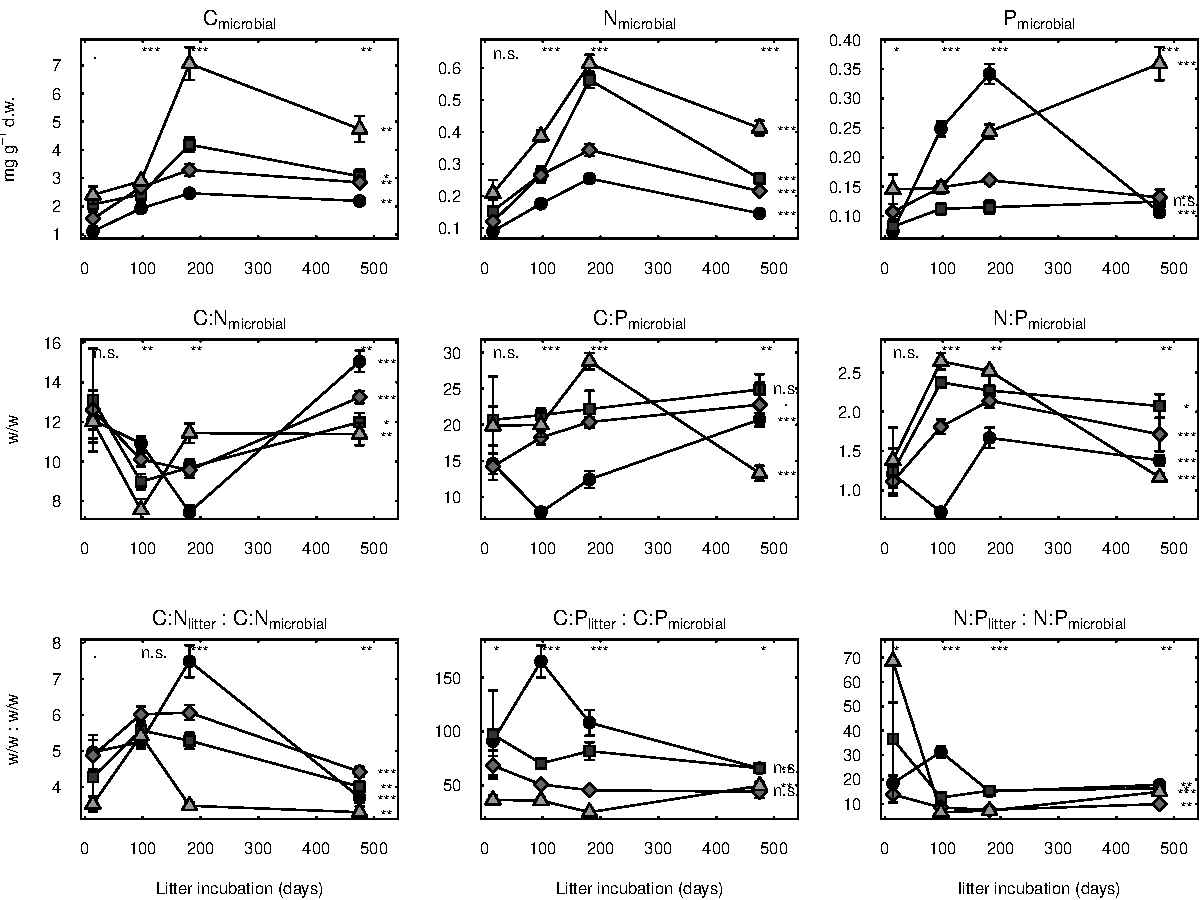
\includegraphics{ligpaper-mb}
\end{center}
%\caption{
%{\bf Microbial biomass C, N and P, microbial C:N:P stoichiometry and resource:consumer stoichiometric imbalance in these elements} in decomposing beech leaf litter from a mesocosm experiment. Beech litter was collected in: triangles, Schottenwald (SW); diamonds, Ossiach (OS); squares, Klausenleopoldsdorf (KL); circles, Achenkirch, AK. Error bars indicate standard errors (n=5). Significant differences between litter types are presented by asterisks above the symbols, significant differences between time points by asterisks to the right of the curves. *, P\textless 0.05, **, P\textless 0.01, ***, P\textless 0.001.}
%\label{fig:mb}
\end{figure}



\newpage
\begin{figure*}[h!]
\vspace*{2mm}
\begin{center}
\setkeys{Gin}{width=\textwidth}
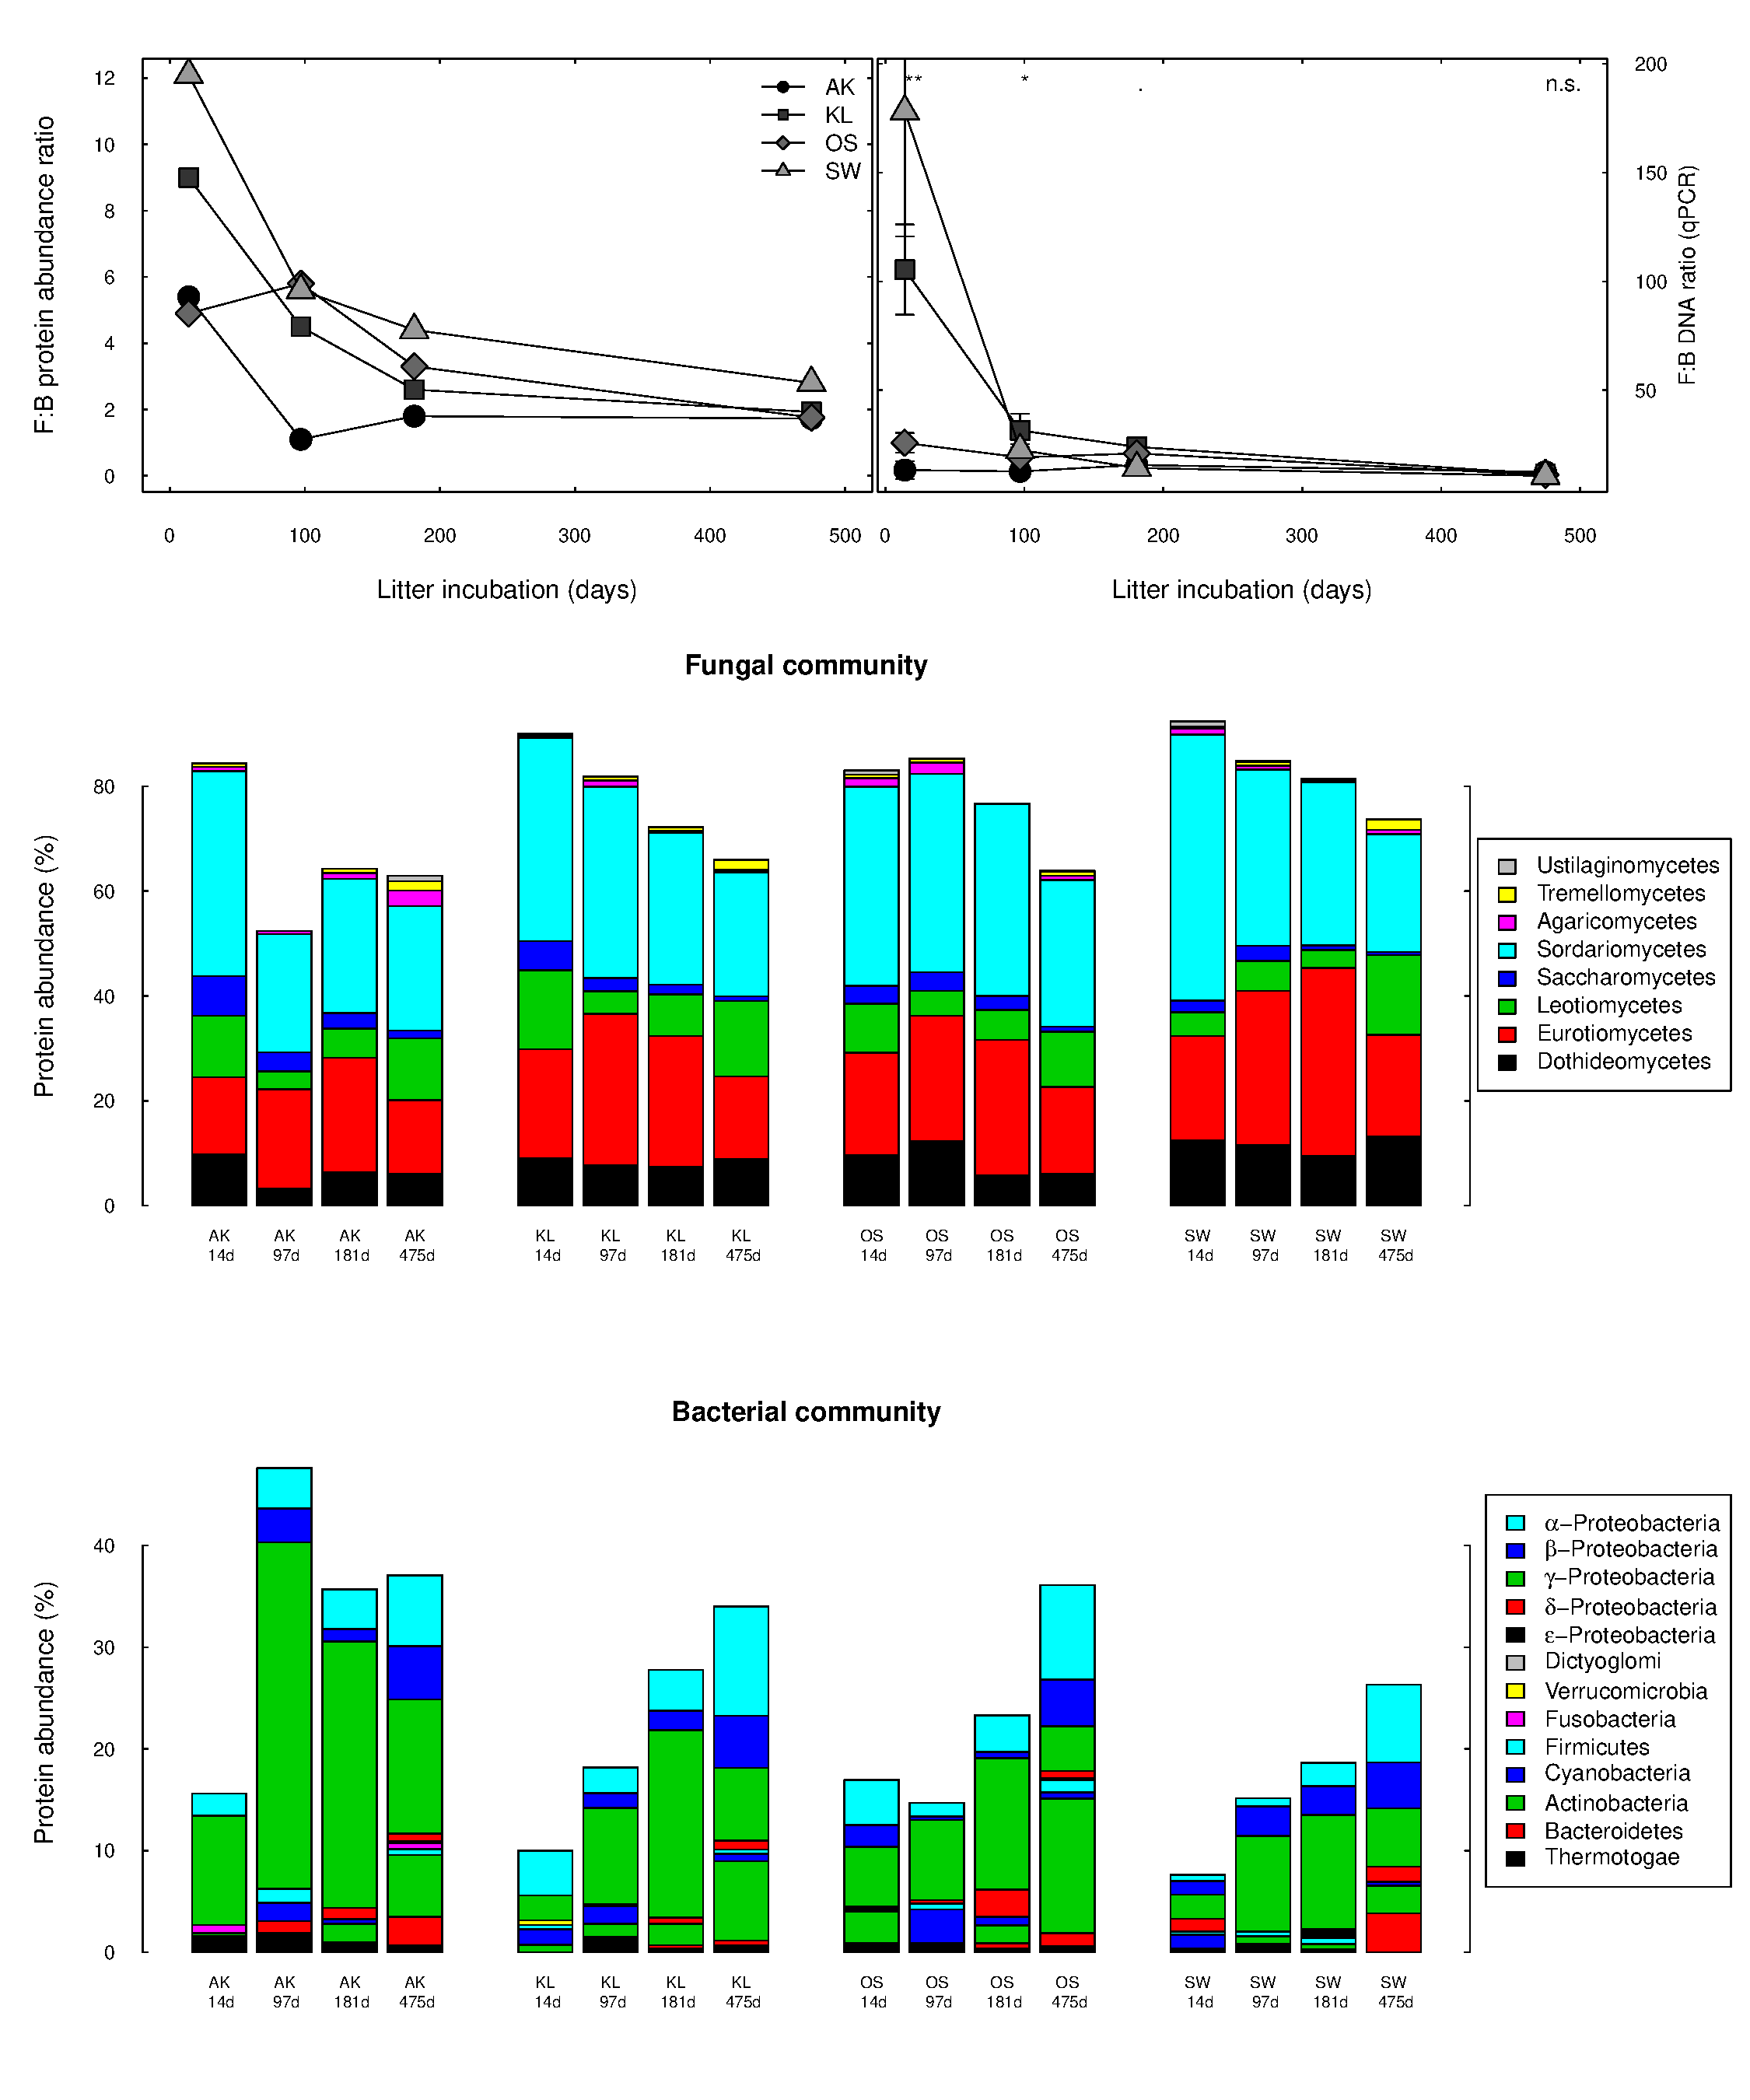
\includegraphics{ligpaper-metaprot2}
\end{center}
%\caption{
%{\bf Protein abundance of fungal and bacterial taxa.} Litter was collected in Achenkirch (AK);, Klausenleopoldsdorf (KL); Ossiach (OS); Schottenwald (SW). Samples were analyzed after sterilization, re-innoculation and incubation for 14, 97, 181, or 475 days.}
%\label{fig:metaprot_barplot}
\end{figure*}


\begin{figure}[!ht]
\begin{center}
\setkeys{Gin}{width=0.7\textwidth}
%\inputgraphics[width=4in]{figure_name.2.eps}
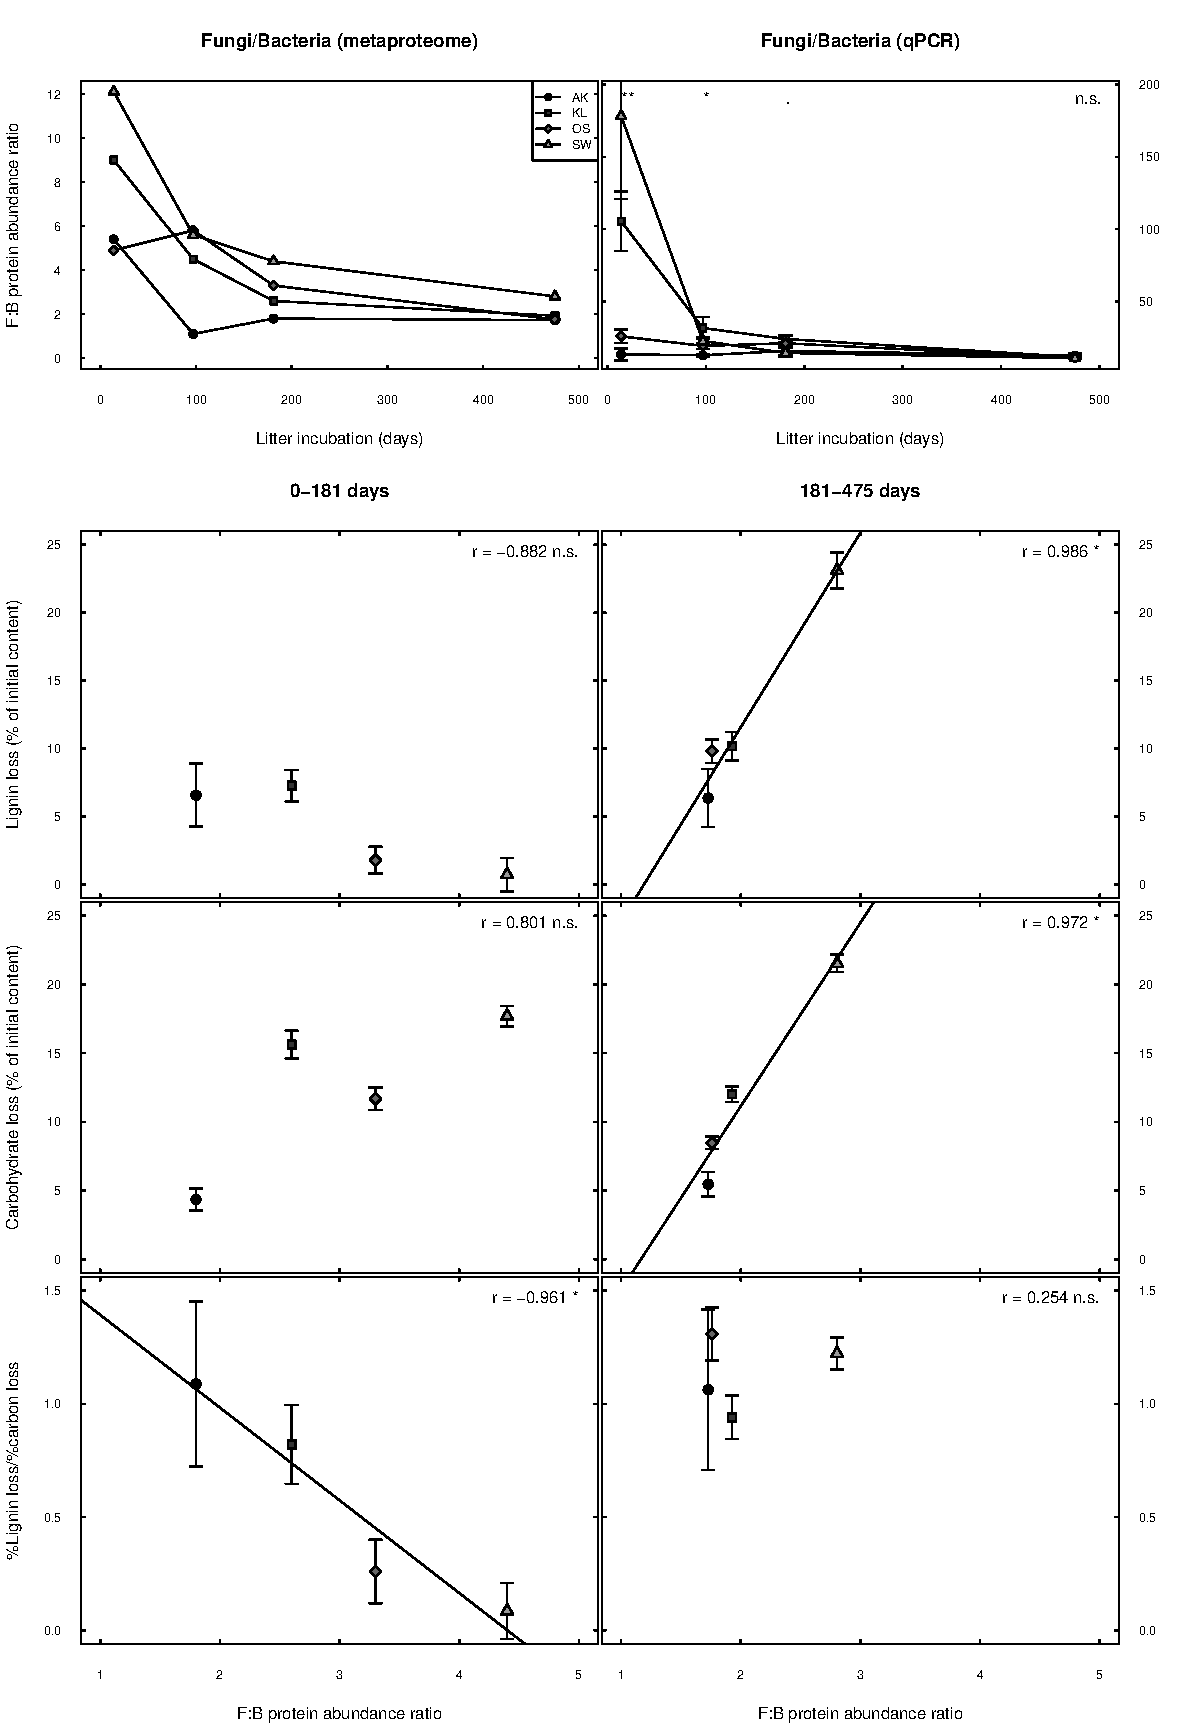
\includegraphics{ligpaper-f2bnew}
\end{center}
%\caption{
%{\bf Fungi:Bacteria (F:B) ratios and their correlations with LCI change:} A: F:B protein abundance (left) and DNA (right) ratio. B: Correlations between F:B preotein abundance ratios and lignin loss (top), carbohydrate loss (mid) and lignin loss : carbon loss (bottom) for 0-6 months (left) and 6-15 months (right, errorbars indicate standard errors, n=4-5).  Beech litter was collected in: triangles, Schottenwald (SW); diamonds, Ossiach (OS); squares, Klausenleopoldsdorf (KL); circles, Achenkirch, AK. Error bars indicate standard errors (n=5). Significant differences between litter types are presented by asterisks above the symbols, significant differences between time points by asterisks to the right of the curves. *, P\textless 0.05, **, P\textless 0.01, ***, P\textless 0.001.}
%\label{fig:f2b}
\end{figure}

\newpage
\begin{figure}[!ht]
\begin{center}
%\setkeys{Gin}{width=4in}
\setkeys{Gin}{width=\textwidth}
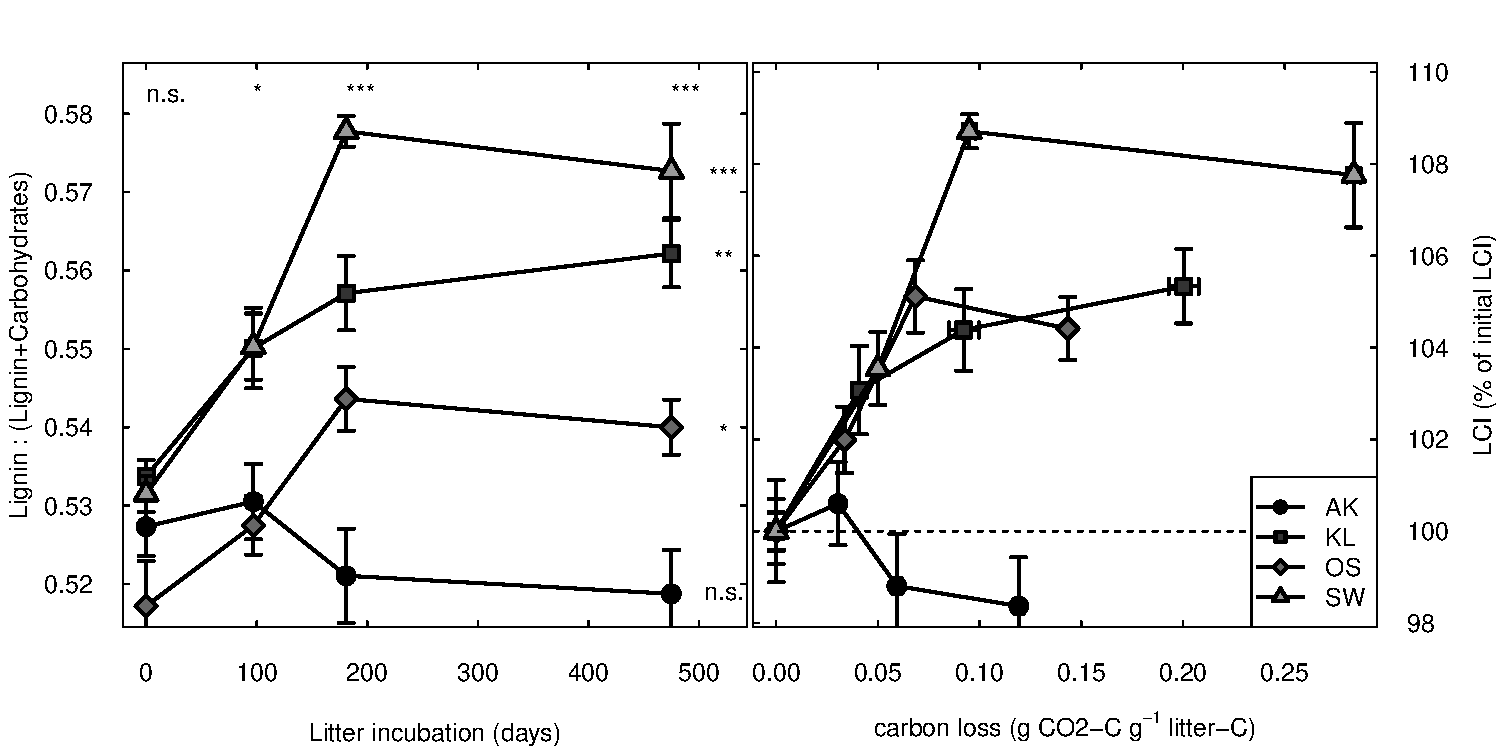
\includegraphics{ligpaper-lci}
\end{center}
%\caption{
%{\bf Develoment of lignin to carbohydrate index (lignin : (lignin+carbohydrates), LCI)} during time of beech litter decomposition (left) or plotted against cumulative C loss (right). Errorbars indicate standard errors (n=4-5). The dashed line indicates a constant ratio between lignin and carbohydrates (i.e. no preferential decomposition of carbohydrates. Beech litter was collected in: triangles, Schottenwald (SW); diamonds, Ossiach (OS); squares, Klausenleopoldsdorf (KL); circles, Achenkirch, AK. Error bars indicate standard errors (n=5). Significant differences between litter types are presented by asterisks above the symbols, significant differences between time points by asterisks to the right of the curves. *, P\textless 0.05, **, P\textless 0.01, ***, P\textless 0.001.}
%\label{fig:lci}
\end{figure}


\newpage
\begin{figure*}[h!]
\vspace*{2mm}
\begin{center}
\setkeys{Gin}{width=\textwidth}
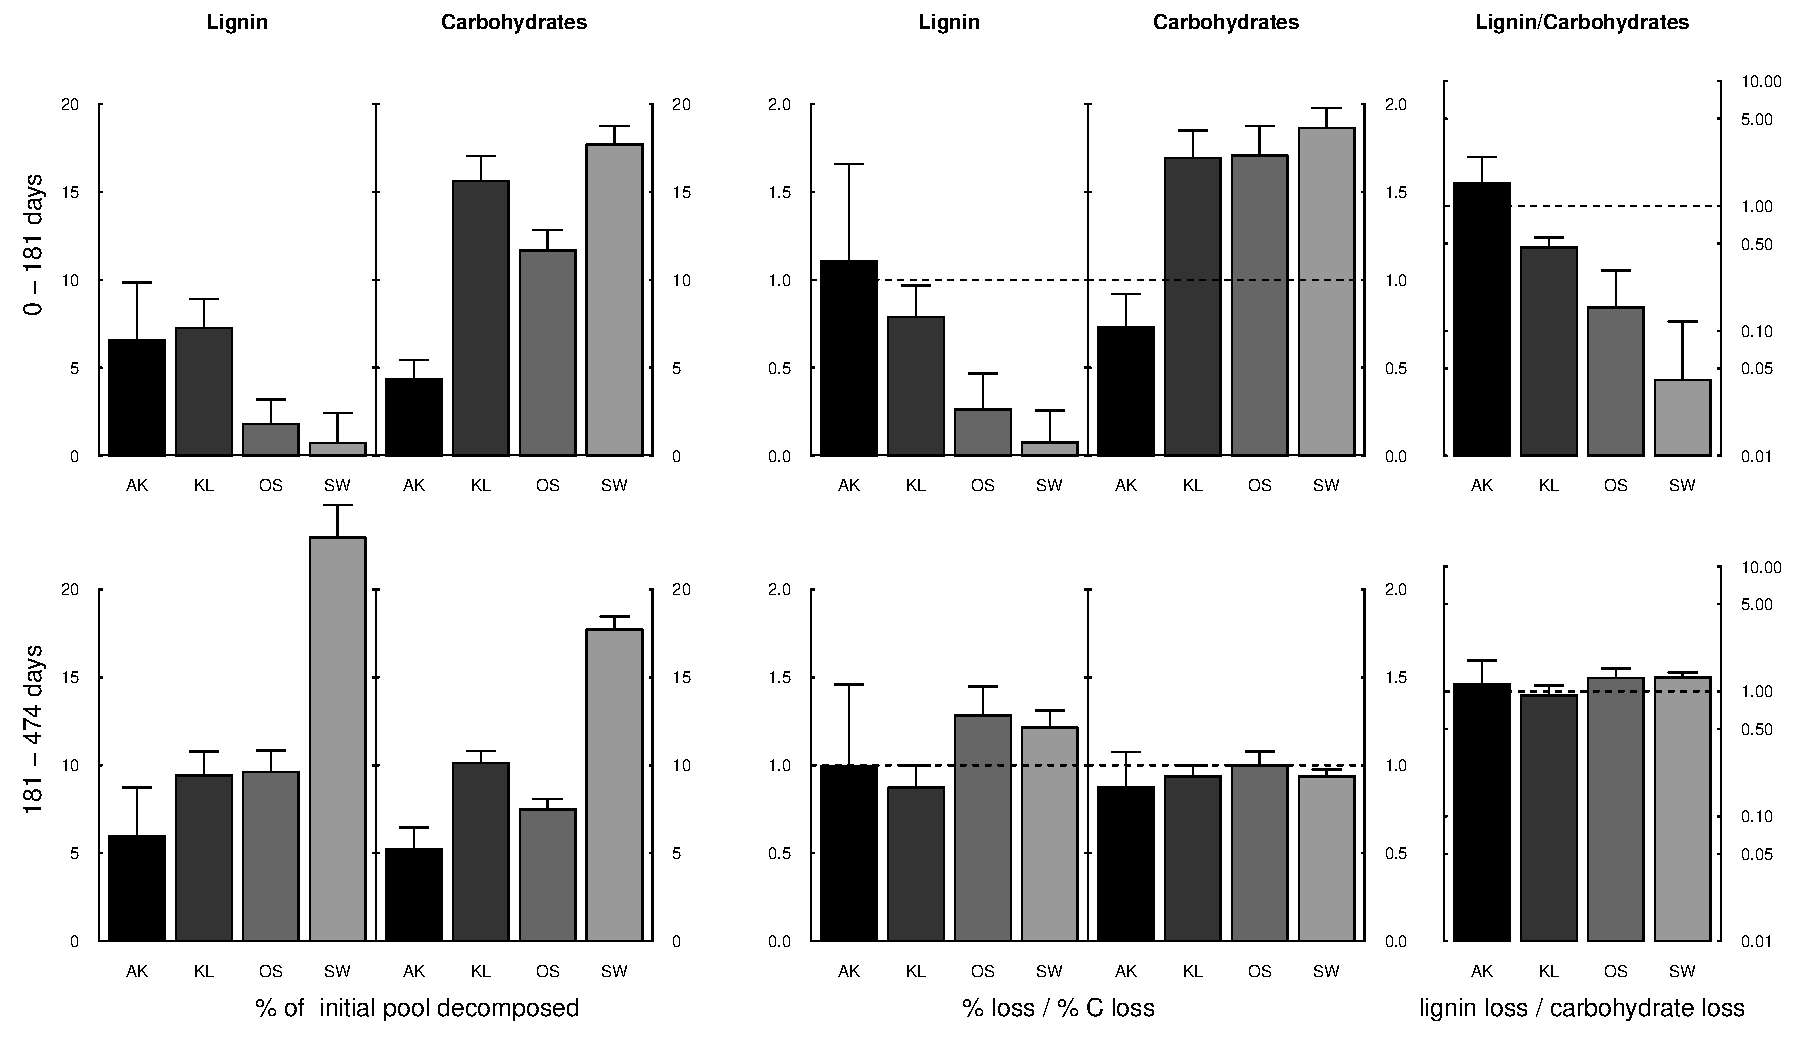
\includegraphics{ligpaper-degrdiff}
\end{center}
%\caption{
%{\bf Carbon loss corrected amounts of lignin and carbohydrates} degraded in beech litter collected in Achenkirch (AK), Klausenleopoldsdorf (KL), Ossiach (OS) and Schottenwald (SW). Carbon loss was calculated based on accumulated respiration for each mesocosm. Error bars indicate standard errors (n=4-5). The dashed line marks no discrimation during decomposition between lignin, carbohydrates and bulk carbon}
%\label{fig:degr}
\end{figure*}

\newpage
\begin{figure*}[h!]
\vspace*{2mm}
\begin{center}
\setkeys{Gin}{width=\textwidth}
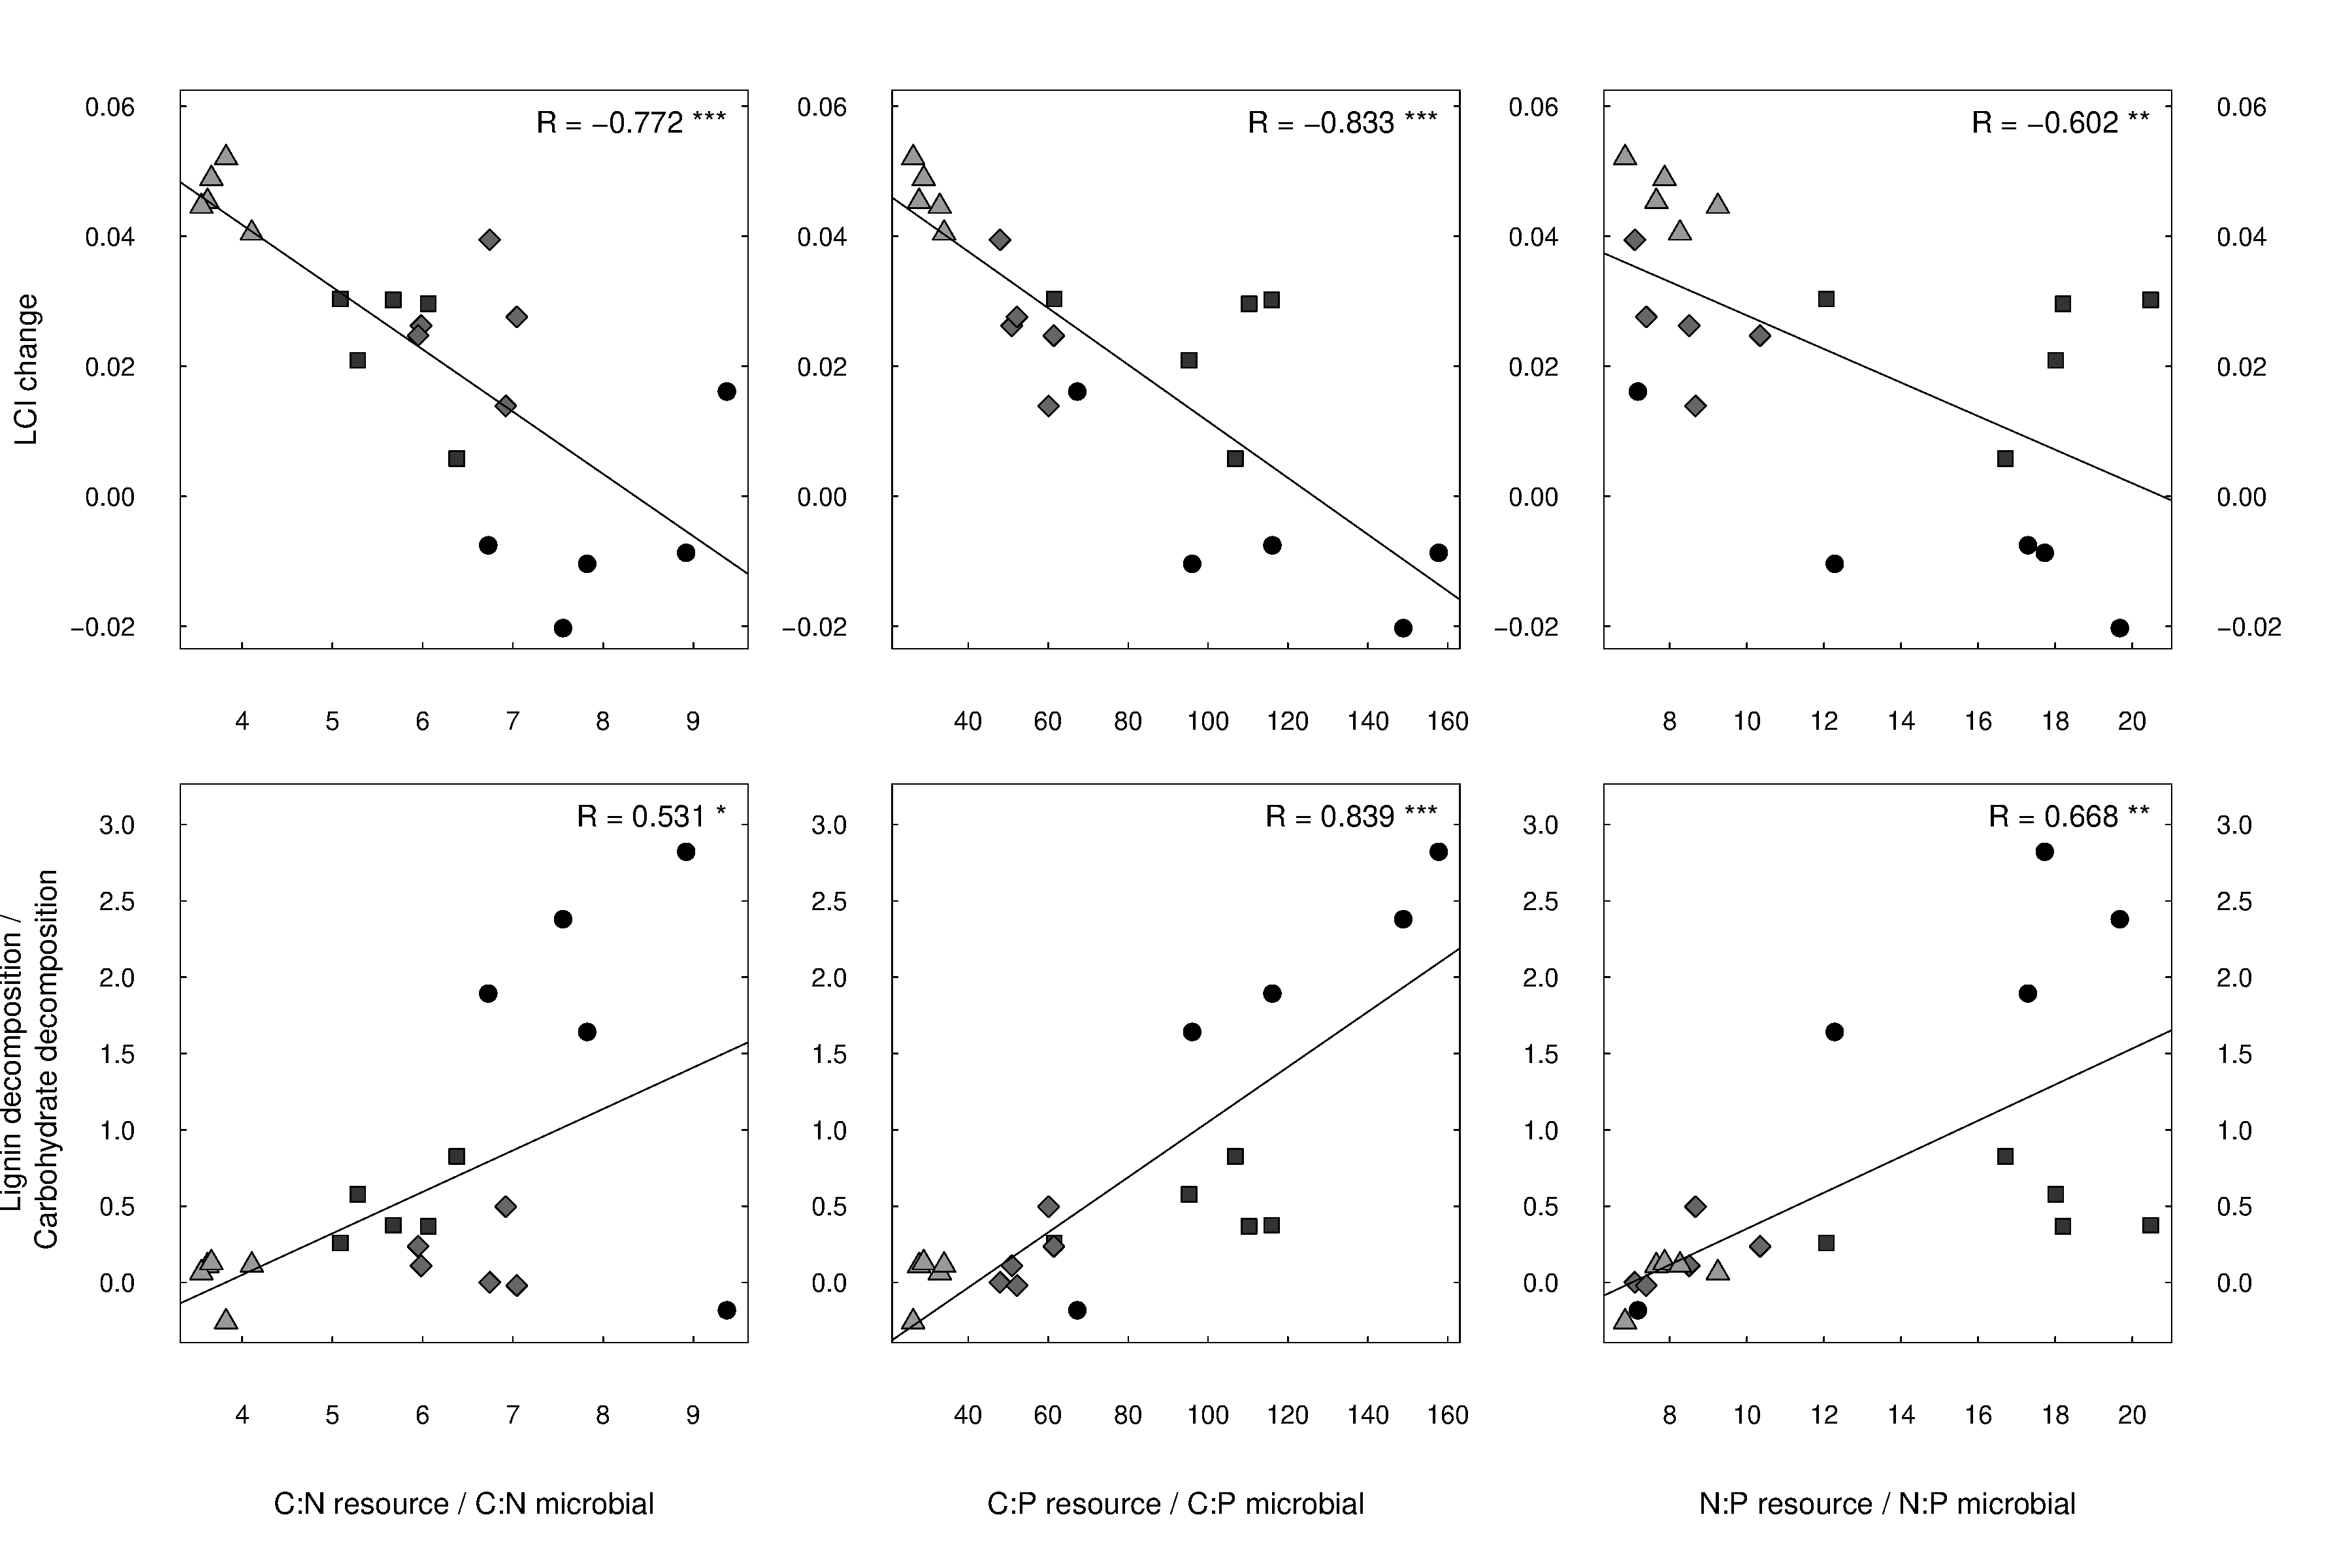
\includegraphics{ligpaper-graphcorr}
\end{center}
%\caption{
%{\bf Correlation between the LCI change or the ratio of lignin : carbohydrate decomposition ratio during the first 6 months of litter decomposition correlate to litter : microbe stoichiometric imbalances.} and change and Correlations between lignin accumulation during the first 6 month of litter incubation and stoichiometric resource:consumer imbalances. LCI is calculates as of lignin/(lignin+Carbohydrates).  Beech litter was collected in: triangles, Schottenwald (SW); diamonds, Ossiach (OS); squares, Klausenleopoldsdorf (KL); circles, Achenkirch, AK. *, P\textless 0.05, **, P\textless 0.01, ***, P\textless 0.001.}
%\label{fig:cor1}
\end{figure*}

\newpage
\begin{figure*}[h!]
\vspace*{2mm}
\begin{center}
\setkeys{Gin}{width=\textwidth}
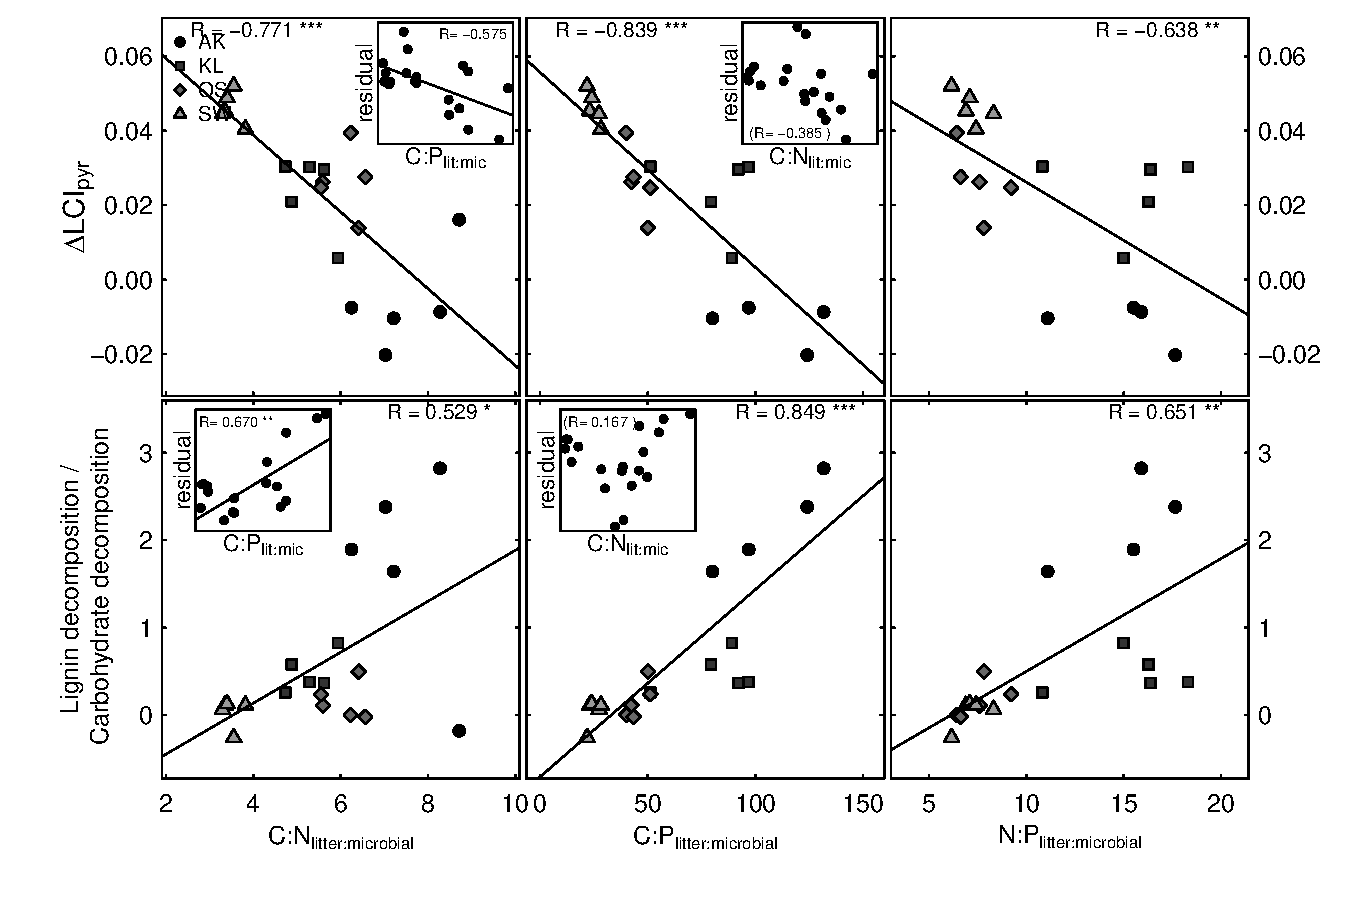
\includegraphics{ligpaper-graphcorr2}
\end{center}
%\caption{
%{\bf Correlation between the LCI change or the ratio of lignin : carbohydrate decomposition ratio during the first 6 months of litter decomposition correlate to litter : microbe stoichiometric imbalances.} and change and Correlations between lignin accumulation during the first 6 month of litter incubation and stoichiometric resource:consumer imbalances. LCI is calculates as of lignin/(lignin+Carbohydrates).  Beech litter was collected in: triangles, Schottenwald (SW); diamonds, Ossiach (OS); squares, Klausenleopoldsdorf (KL); circles, Achenkirch, AK. *, P\textless 0.05, **, P\textless 0.01, ***, P\textless 0.001.}
%\label{fig:cor1}
\end{figure*}


%\SweaveInput{metaprot_calc}


\newpage
\begin{figure*}[h!]
\vspace*{2mm}
\begin{center}
\setkeys{Gin}{width=\textwidth}
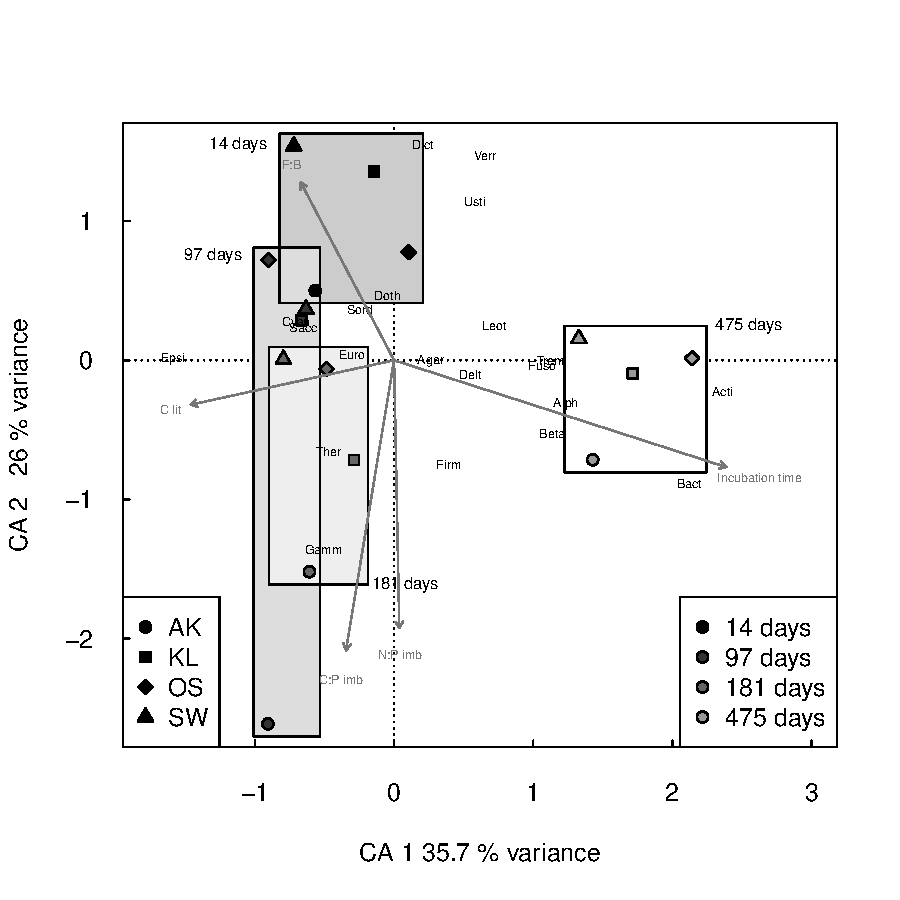
\includegraphics{ligpaper-metaprot_pca}
\end{center}
%\caption{
%{\bf Microbial commuity composition.} The first two components of a correspondance analysis (CA) of protein abundances found. Rectangles indicate samples of identical incubation time. Peptides were aggregated at class level (fungi and proteobacteria) or phylum level (other bacterial phyla): Dothideomycetes (Doth); Eurotiomycetes (Euro); Leotiomycetes (Leot); Saccharomycetes (Sacc); Sordariomycetes (Sord); Agaricomycetes (Agar); Tremellomycetes (Trem); Ustilaginomycetes (Usti); Thermotogae (Ther); Bacteroidetes (Bact); Actinobacteria (Acti); Cyanobacteria (Cyan); Firmicutes (Firm); Fusobacteria (Fuso); Verrucomicrobia (Verr); Dictyoglomi (Dict); Alphaproteobacteria (Alph); Betaproteobacteria (Beta); Gammaproteobacteria (Gamm); Deltaproteobacteria (Delt); Epsilonproteobacteria (Epsi). Taxa factor loadings were printed x2 for better readability. Correlations between CA 1, CA 2, and litter chemistry, microbial stoichiometry, and protein abundance of microbial taxa are stated in supplemental table \ref{catab}. 
%Arrows represent vectorial fittings of these variables calculated independently from the CA, plotted only if p\textless 0.05: Litter C content (C lit); C:X\textsubscript{Microbial}/C:X\textsubscript{Litter} (C:P imb, C:N imb).}
%\label{fig:metaprotpca}
\end{figure*}

\newpage
%\section*{Tables}

%\begin{landscape}
% latex table generated in R 2.12.1 by xtable 1.5-6 package
% Sat Nov  5 23:56:54 2011
\begin{table}[h!]
%\begin{center}
\caption{Element concentrations, elemental stoichiometry and cellulose and lignin concentrations in beech litter measured after 14 days incubation. Standard errors are given in brackets (n=5). C extr represents for soluble organic carbon. Beech litter was collected in AK, Achenkirch, KL, Klausenleopoldsdorf, OS, Ossiach, and SW, Schottenwald.}
\label{initstoech}

{\small
\begin{tabular}{lrlrlrlrlrlr}
  \hline
 & AK & (SE) & KL & (SE) & OS & (SE) & SW & (SE) & p value \\ 
  \hline
C (\% d.w.) & 50.86 & (0.39) & 49.41 & (0.53) & 48.15 & (0.39) & 48.90 & (0.34) & 0.002 \\ 
  C extr (mg g-1) & 0.46 & (0.03) & 0.14 & (0.01) & 0.21 & (0.01) & 0.64 & (0.03) & $<$0.001 \\ 
  N (\% d.w.) & 0.878 &  (0.012) & 0.938 &  (0.012) & 0.806 &  (0.013) & 1.172 &  (0.016) & $<$0.001 \\ 
  P (\% d.w.) & 0.040 & (0.000) & 0.030 & (0.000) & 0.052 & (0.002) & 0.070 & (0.000) & $<$0.001 \\ 
  C:N (w/w) & 57.86 &  (0.57) & 52.60 &  (0.49) & 59.97 &  (0.72) & 41.78 &  (0.76) & $<$0.001 \\ 
  C:P (w/w) & 1282 & (21) & 1548 & (25) & 905 & (15) & 699 & (9) & $<$0.001 \\ 
  N:P (w/w) & 22.17 & (0.47) & 29.45 & (0.60) & 15.10 & (0.29) & 16.75 & (0.39) & $<$0.001 \\ 
  K (mg g-1) & 0.26 & (0.00) & 0.54 & (0.00) & 0.21 & (0.00) & 0.55 & (0.00) & $<$0.001 \\ 
  Ca (mg g-1) & 1.33 & (0.01) & 1.26 & (0.01) & 1.63 & (0.01) & 1.23 & (0.01) & $<$0.001 \\ 
  Mg (mg g-1) & 0.27 &  (0.00) & 0.14 &  (0.00) & 0.20 &  (0.00) & 0.15 &  (0.00) & $<$0.001 \\ 
  Fe (ppm) & 210 & (2) & 208 & (4) & 453 & (12) & 192 & (4) & $<$0.001 \\ 
  Mn (ppm) & 172 &  (2) & 1430 &  (10) & 776 &  (9) & 2137 &  (51) & $<$0.001 \\ 
  Zn (ppm) & 30.8 & (0.4) & 33.0 & (0.3) & 36.0 & (1.0) & 42.4 & (0.7) & $<$0.001 \\ 
  Lignin & 28.9 & (28.9) & 29.9 & (29.9) & 31.2 & (31.2) & 30.5 & (30.5) & $<$0.001 \\ 
  Carbohydrates & 25.9 & (25.9) & 26.1 & (26.1) & 29.2 & (29.2) & 26.9 & (26.9) & $<$0.001 \\ 
   \hline
\end{tabular}
}
%\end{center}
\end{table}
\end{landscape}




%\section*{Supporting Information}


%\begin{landscape}
% latex table generated in R 2.12.1 by xtable 1.5-6 package
% Sat Nov  5 23:56:54 2011
\begin{table}[h!]
%\begin{center}
\caption{Element concentrations, elemental stoichiometry and cellulose and lignin concentrations in beech litter measured after 14 days incubation. Standard errors are given in brackets (n=5). C extr represents for soluble organic carbon. Beech litter was collected in AK, Achenkirch, KL, Klausenleopoldsdorf, OS, Ossiach, and SW, Schottenwald.}
\label{initstoech}

{\small
\begin{tabular}{lrlrlrlrlrlr}
  \hline
 & AK & (SE) & KL & (SE) & OS & (SE) & SW & (SE) & p value \\ 
  \hline
C (\% d.w.) & 50.86 & (0.39) & 49.41 & (0.53) & 48.15 & (0.39) & 48.90 & (0.34) & 0.002 \\ 
  C extr (mg g-1) & 0.46 & (0.03) & 0.14 & (0.01) & 0.21 & (0.01) & 0.64 & (0.03) & $<$0.001 \\ 
  N (\% d.w.) & 0.878 &  (0.012) & 0.938 &  (0.012) & 0.806 &  (0.013) & 1.172 &  (0.016) & $<$0.001 \\ 
  P (\% d.w.) & 0.040 & (0.000) & 0.030 & (0.000) & 0.052 & (0.002) & 0.070 & (0.000) & $<$0.001 \\ 
  C:N (w/w) & 57.86 &  (0.57) & 52.60 &  (0.49) & 59.97 &  (0.72) & 41.78 &  (0.76) & $<$0.001 \\ 
  C:P (w/w) & 1282 & (21) & 1548 & (25) & 905 & (15) & 699 & (9) & $<$0.001 \\ 
  N:P (w/w) & 22.17 & (0.47) & 29.45 & (0.60) & 15.10 & (0.29) & 16.75 & (0.39) & $<$0.001 \\ 
  K (mg g-1) & 0.26 & (0.00) & 0.54 & (0.00) & 0.21 & (0.00) & 0.55 & (0.00) & $<$0.001 \\ 
  Ca (mg g-1) & 1.33 & (0.01) & 1.26 & (0.01) & 1.63 & (0.01) & 1.23 & (0.01) & $<$0.001 \\ 
  Mg (mg g-1) & 0.27 &  (0.00) & 0.14 &  (0.00) & 0.20 &  (0.00) & 0.15 &  (0.00) & $<$0.001 \\ 
  Fe (ppm) & 210 & (2) & 208 & (4) & 453 & (12) & 192 & (4) & $<$0.001 \\ 
  Mn (ppm) & 172 &  (2) & 1430 &  (10) & 776 &  (9) & 2137 &  (51) & $<$0.001 \\ 
  Zn (ppm) & 30.8 & (0.4) & 33.0 & (0.3) & 36.0 & (1.0) & 42.4 & (0.7) & $<$0.001 \\ 
  Lignin & 28.9 & (28.9) & 29.9 & (29.9) & 31.2 & (31.2) & 30.5 & (30.5) & $<$0.001 \\ 
  Carbohydrates & 25.9 & (25.9) & 26.1 & (26.1) & 29.2 & (29.2) & 26.9 & (26.9) & $<$0.001 \\ 
   \hline
\end{tabular}
}
%\end{center}
\end{table}
\end{landscape}

\begin{table}[h!]
\begin{center}
\caption{Lignin derrived and other phenolic pyrolysis products}
\label{tab:phprod}

{\small
\begin{tabular}{lcccccc}
  \hline
Name & RT & MW & integrated framents & Origin & Class \\ 
  \hline
Guaiacol & 18.87 & 124 & 109+124 &Lignin&Guaiacyl\\ 
Methylguaiacol & 20.32 & 138 & 123+138 &Lignin&Guaiacyl\\ 
Ethylguaiacol & 21.40 & 152 & 137+152 &Lignin&Guaiacyl\\ 
Propenylguaiacol & 23.29 & 164 & 149+164 &Lignin&Guaiacyl\\ 
Vinylguaiacol & 23.69 & 150 & 135+150 &Lignin&Guaiacyl\\ 
Propenylguaiacol & 24.48 & 164 & 149+164 &Lignin&Guaiacyl\\ 
Syringol & 24.58 & 154 & 139+154 &Lignin&Syringyl\\ 
Propenylguaiacol & 25.66 & 164 & 149+164 &Lignin&Guaiacyl\\ 
Methylsyringol & 25.67 & 168 & 153+168 &Lignin&Syringyl\\ 
Ethylsysringol & 26.39 & 182 & 167+182 &Lignin&Syringyl\\ 
Propenylsyringol & 27.97 & 194 & 179+194 &Lignin&Syringyl\\ 
Vinylsyringol & 28.37 & 180 & 165+180 &Lignin&Syringyl\\ 
Guaiacolaldehyde & 28.40 & 152 & 109+152 &Lignin&Guaiacyl\\ 
Propylguaiacol & 28.72 & 166 & 137+166 &Lignin&Guaiacyl\\ 
Oxo-hydroxy-etylguaiacol & 28.77 & 182 & 182 &Lignin&Guaiacyl\\ 
Propenylsyringol & 28.91 & 194 & 179+194 &Lignin&Syringyl\\ 
Oxo-ethylguaiacol & 29.20 & 166 & 151+166 &Lignin&Guaiacyl\\ 
Oxo-propylguaiacol & 29.36 & 180 & 137+180 &Lignin&Guaiacyl\\ 
Propenylsyringol & 30.16 & 194 & 194+179 &Lignin&Syringyl\\ 
Syringolaldehyde & 32.68 & 182 & 139+182 &Lignin&Syringyl\\ 
Oxo-hydroxy-ethylsyringol & 32.80 & 212 & 212 &Lignin&Syringyl\\ 
Guaiacolacetic acid & 32.88 & 182 & 137+182 &Lignin&Guaiacyl\\ 
Propylsyringol & 33.15 & 196 & 181+196 &Lignin&Syringyl\\ 
Oxo-propylsyringol & 33.32 & 210 & 167+210 &Lignin&Syringyl\\ 
Oxopropenylguaiacol & 35.30 & 178 & 135+178 &Lignin&Guaiacyl\\ 
Hydroxypropenylguaiacol & 37.10 & 180 & 137+180 &Lignin&Guaiacyl\\ 
Syringolacetic acid & 38.78 & 212 & 212 &Lignin&Syringyl\\ 
Oxo-propenylsyringol & 43.06 & 208 & 165+208 &Lignin&Syringyl\\ 
Phenol & 21.02 & 94 & 65+66+94 &Phenolic&\\ 
4-Methylphenol & 22.11 & 108 & 107+108 &Phenolic&\\ 
3-Methylphenol & 22.22 & 108 & 107+108 &Phenolic&\\ 
Ethylphenol & 23.38 & 122 & 107+122 &Phenolic&\\ 
Propenylphenol & 26.93 & 134 & 133+134 &Phenolic&\\ 
Propenylphenol & 27.76 & 134 & 133+134 &Phenolic&\\ 
Propylphenol & 31.11 & 136 & 151+166 &Phenolic&\\ 
Butylphenol & 31.86 & 150 & 107+150 &Phenolic&\\ 
4-Hydroxybenzaldehyde & 32.70 & 122 & 121+122 &Phenolic&\\ 
Hydroquinone & 33.40 & 110 & 81+110 &Phenolic&\\ 
   \hline
\end{tabular}
}
\end{center}
\end{table}
\newpage

% latex table generated in R 2.12.1 by xtable 1.6-0 package
% Tue Nov  8 06:46:38 2011
\begin{table}[h!]
\begin{center}
\caption{Carbohydrate derrived pyrolysis products}
\label{tab:chprod}
{\small
\begin{tabular}{lcccccc}
  \hline
Name & RT & MW & integrated framents & Origin & Class \\ 
  \hline
Acetaldehyde & 2.06 & 44 & 29+44 &Carbohydrates&  \\ 
Furan & 2.35 & 68 & 39+68 &Carbohydrates&Furan\\ 
Methylfuran & 2.74 & 82 & 81+82 &Carbohydrates&Furan\\ 
Methylfuran & 2.91 & 82 & 81+82 &Carbohydrates&Furan\\ 
Dimethylfuran & 3.43 & 96 & 95+96 &Carbohydrates&Furan\\ 
Dimethylfuran & 3.66 & 96 & 95+96 &Carbohydrates&Furan\\ 
Vinylfuran & 5.01 & 94 & 65+94 &Carbohydrates&Furan\\ 
Unknown furan & 6.36 & 108 & 107+108 &Carbohydrates&Furan\\ 
Cyclopentanone & 6.99 & 105? & 84+105? &Carbohydrates&Cyclopentenone\\ 
Methylfuran & 7.62 & 82 & 53+82+83 &Carbohydrates&Furan\\ 
2-Oxopropanoic acid, methylester & 7.92 & 102 & 43+102 &Carbohydrates& \\ 
1-Hydroxypropanone & 9.24 & 74 & 43 &Carbohydrates& \\ 
2-Cyclopenten-1-one & 10.26 & 82 & 53+54+52 &Carbohydrates&Cyclopentenone\\ 
2-Methyl-2-cyclopenten-1-one & 10.51 & 96 & 53+96 &Carbohydrates&Cyclopentenone\\ 
1-Hydroxy-2-propanone & 10.69 & 88 & 57+88 &Carbohydrates&Cyclopentenone\\ 
Unknown & 11.38 & unk & 65+66+94 &Carbohydrates& \\ 
3-Furaldehyd & 11.57 & 96 & 95+96 &Carbohydrates&Furan\\ 
2(5H)Furanon & 11.69 & 98 & 55+98 &Carbohydrates&Furan\\ 
Propanoic acid, methylester & 12.10 & 102 & 43+102 &Carbohydrates& \\ 
2-Furaldehyd & 12.22 & 96 & 95+96 &Carbohydrates&Furan\\ 
Acetylfuran & 12.99 & 110 & 95+110 &Carbohydrates&Cyclopentenone\\ 
3-Methyl-cyclopentanone & 13.31 & 96 & 67+96 &Carbohydrates&Cyclopentenone\\ 
Dimethylcyclopentenone & 13.69 & 110 & 67+95+110 &Carbohydrates&Cyclopentenone\\ 
5-Methyl-2-furancarboxaldehyde & 14.23 & 110 & 109+110 &Carbohydrates&Furan\\ 
2-Cyclopenten-1,4-dione & 14.44 & 96 & 54+68+96 &Carbohydrates&Cyclopentenone\\ 
Butyrolactone & 15.22 & 86 & 56+86 &Carbohydrates& \\ 
Unknown & 15.56 &  &  &Carbohydrates&  \\ 
Furanmethanol & 15.61 & 98 & 98 &Carbohydrates&Cyclopentenone\\ 
5-Methyl-2(5H)-furanone & 16.06 & 98 & 55+98 &Carbohydrates&Furan\\ 
Unknown & 16.17 & unk & 110 &Carbohydrates&  \\ 
1,2-Cylopentandione & 17.51 & 98 & 55+98 &Carbohydrates&Cyclopentenone\\ 
Unknown & 17.67 & unk & 42+70 &Carbohydrates&  \\ 
2-Hydroxy-3-methyl-2-cyclopenten-1-one & 18.14 & 98 & 98 &Carbohydrates&Cyclopentenone\\ 
3-Methy-l1,2-cyclopentanedione & 18.42 & 112 & 69+112 &Carbohydrates&Cyclopentenone\\ 
Unknown & 19.06 && 58+86+114 &Carbohydrates&\\ 
Unknown & 19.35 && 98+126 &Carbohydrates&\\ 
Unknown & 21.77 && 116 &Carbohydrates&\\ 
Unknown & 22.33 && 44 &Carbohydrates&\\ 
Unknown & 26.18 && 57+69 &Carbohydrates&\\ 
5-Hydroxymethylfuran-1-carboxaldehyde & 27.51 & 126 & 97+126 &Carbohydrates&Furan\\ 
Unknown & 31.67 && 73+135 &Carbohydrates&\\ 
Laevoglucosan & 40.44 & 172 & 60+73 &Carbohydrates& \\ 
   \hline
\end{tabular}
}
\end{center}
\end{table}


\newpage
% latex table generated in R 2.12.1 by xtable 1.6-0 package
% Tue Nov  8 06:46:38 2011
\begin{table}[h!]
\begin{center}
\caption{Other pyrolysis products quantified}
\label{tab:nprod}
{\small
\begin{tabular}{lcccccc}
  \hline
Name & RT & MW & integrated framents & Origin & Class \\ 
  \hline
25:0 Alkan & 27.74 & 352 & 57+71 &aliphatic& Alkan \\ 
25:1 Alken & 28.34 & 350 & 57+69 &aliphatic& Alken \\ 
27:0 Alkan & 30.04 & 380 & 57+67 &aliphatic& Alkan \\ 
27:1 Alken & 30.63 & 378 & 57+65 &aliphatic& Alken \\ 
29:0 Alkan & 32.20 & 408 & 57+63 &aliphatic& Alkan \\ 
29:1 Alken & 32.82 & 406 & 57+61 &aliphatic& Alken \\ 
Myristic acid (14:0) & 2.35 & 68 & 39+68 & Lipid & Fatty Acid \\ 
Palmitic acid (16:0) & 2.74 & 82 & 81+82 & Lipid & Fatty Acid \\ 
Stearuc acid (18:0) & 2.91 & 82 & 81+82 & Lipid & Fatty Acid \\ 
N-methyl-pyrrol & 6.15 & 81 & 80+81 &Protein& Pyrrol \\ 
Pyridine & 6.90 & 95 & 52+79+95 &Protein& Pyridine \\ 
Methylpyridine & 7.50 & 93 & 66+92+93 &Protein& Pyridine \\ 
Methylpyridine & 7.54 & 93 & 66+92+93 &Protein& Pyridine \\ 
methylpyridine & 9.02 & 93 & 66+93 &Protein& Pyridine \\ 
Pyrrol & 13.11 & 67 & 39+41+67 &Protein& Pyrrol \\ 
Methylpyrrol & 13.81 & 81 & 80+81 &Protein& Pyrrol \\ 
Methylpyrrol & 14.10 & 81 & 80+81 &Protein& Pyrrol \\ 
3-Hydroxypyridine & 26.52 & 95 & 67+95 &Protein& Pyridine \\ 
Indole & 26.85 & 117 & 89+117 &Protein& Indole \\ 
Methylindole & 27.42 & 131 & 130+131 &Protein& Indole \\ 
Toluene & 4.54 & 92 & 91+92 &&Aromatic\\ 
Xylene & 5.94 & 106 & 91+105+106 &&Aromatic\\ 
Xylene & 6.09 & 106 & 91+105+106 &&Aromatic\\ 
Xylene & 6.20 & 106 & 91+105+106 &&Aromatic\\ 
Xylene & 6.99 & 105? & 84+105? &&Aromatic\\ 
Methoxytoluene & 11.78 & 122 & 121+122 &&Aromatic\\ 
Indene & 12.64 & 116 & 115+116 &&Aromatic\\ 
Benzaldehyde & 13.35 & 106 & 77+106 &&Aromatic\\ 
Dihydrobenzofuran & 26.19 & 120 & 91+119+120 &  & Aromatic \\ 
Limonene & 7.22 & 136 & 93 && Terpene \\ 
Phytol & 20.00 & 276 & 95+123 & Chlorophyll & Terpene \\ 
Unknown aliphatic & 22.82 && 58+71 && aliphatic \\ 
Aceton & 2.46 & 58 & 43 &  &  \\ 
2-Propenal & 2.60 & 56 & 55+56 &  &\\ 
Methanol & 2.88 & 32 & 29+31+32 &  &\\ 
3-Buten-2-one & 3.39 & 70 & 55+70 &  &\\ 
2,3-Butandione & 3.67 & 86 & 69+86 &&\\ 
3-Penten-2-one & 3.89 & 86 & 69+86 &&\\ 
2-Butanal & 4.56 & 70 & 69+70 &&\\ 
2,3-Pentadione & 4.77 & 100 & 57+100 &&\\ 
Hexanal & 5.16 & 82 & 56+72+82 &&\\ 
1-Penten-3-one & 11.28 & 84 & 55+84 &&\\ 
Hexan-2,4-dion & 23.92 & 114 & 56+84+114 &&  \\ 
unknown & 15.98 && 119+134 &&\\ 
Unknown & 20.85 && 81 &&\\ 
Unknown & 20.86 && 82+95 &&\\ 
Unknown & 22.43 && 98+128 &&\\ 
Unknown & 27.76 && 138 &&\\ 
   \hline
\end{tabular}
}
\end{center}
\end{table}


% latex table generated in R 2.15.2 by xtable 1.7-1 package
% Wed Nov 13 18:36:18 2013
\begin{table}[h!]
\centering
\caption{caption} 
\label{cor_pyrpca}
{\small
\begin{tabular}{lrrr}
  \hline
 & PC1 & PC2 & PC3 \\ 
  \hline
al & \textbf{ 0.867 } & 0.029 & 0.018 \\ 
  C & \textbf{ -0.414 } & \textbf{ -0.813 } & 0.009 \\ 
  L & \textbf{ 0.572 } & \textbf{ -0.693 } & -0.145 \\ 
  lip & 0.034 & 0.181 & -0.138 \\ 
  N & \textbf{ 0.663 } & 0.227 & \textbf{ -0.293 } \\ 
  non & \textbf{ 0.644 } & 0.025 & -0.112 \\ 
  Ph & -0.197 & \textbf{ 0.922 } & 0.113 \\ 
  phytol & -0.001 & \textbf{ 0.396 } & \textbf{ -0.266 } \\ 
  unk & \textbf{ -0.808 } & \textbf{ 0.388 } & 0.157 \\ 
  al   & \textbf{ 0.779 } & \textbf{ 0.286 } & \textbf{ 0.290 } \\ 
  al0   & \textbf{ 0.793 } & 0.063 & 0.063 \\ 
  al1   & \textbf{ 0.917 } & -0.067 & -0.105 \\ 
  ar   & \textbf{ 0.229 } & \textbf{ 0.543 } & \textbf{ -0.674 } \\ 
  bf   & \textbf{ -0.793 } & \textbf{ 0.412 } & 0.144 \\ 
  cp   & \textbf{ 0.937 } & -0.166 & 0.066 \\ 
  f   & \textbf{ -0.807 } & \textbf{ -0.494 } & \textbf{ -0.241 } \\ 
  fa   & 0.034 & 0.181 & -0.138 \\ 
  g   & \textbf{ 0.545 } & \textbf{ -0.737 } & -0.045 \\ 
  ind   & \textbf{ 0.628 } & \textbf{ 0.564 } & -0.221 \\ 
  N-me-pyr   & \textbf{ 0.506 } & -0.049 & \textbf{ -0.818 } \\ 
  o   & 0.013 & -0.203 & \textbf{ 0.408 } \\ 
  p   & \textbf{ 0.719 } & \textbf{ 0.358 } & \textbf{ -0.416 } \\ 
  ph   & -0.197 & \textbf{ 0.922 } & 0.113 \\ 
  phytol   & -0.001 & \textbf{ 0.396 } & \textbf{ -0.266 } \\ 
  pyridol   & \textbf{ 0.272 } & -0.123 & 0.009 \\ 
  s   & \textbf{ 0.878 } & -0.137 & \textbf{ 0.408 } \\ 
  short   & \textbf{ 0.695 } & -0.217 & 0.195 \\ 
  sy   & \textbf{ 0.552 } & \textbf{ -0.508 } & \textbf{ -0.332 } \\ 
  ter   & \textbf{ -0.882 } & 0.186 & \textbf{ -0.230 } \\ 
  unk   & \textbf{ -0.776 } & \textbf{ -0.522 } & 0.089 \\ 
   \hline
\end{tabular}
}
\end{table}


\begin{landscape}

% latex table generated in R 2.15.2 by xtable 1.7-1 package
% Wed Nov 13 18:36:18 2013
\begin{table}[h!]
\centering
\caption{Results of correlation analysis (R) between lignin and carbohydrate decomposition and other decomposition processes (mass loss, respiration), extracellular enzyme activities, litter chemistry, and litter and microbial biomass C:N:P stoichiometry. Significant (p\textless 0.05) correlations are presented in bold. Changes in litter chemistry (lignin and carbohydrate decomposition) were calculated between 0 and 181 days, other data were measured after 181 days. $\Delta LCI_{pyr}$ - difference in the pyr-GC/MS based lignocellulose index (lignin:(lignin + carbohydrates)), $L_{degr}$, $Ch_{degr}$ - \% of initial lignin or carbohydrate loss, $L/C_{degr}$, $Ch/C_{degr}$  - \% lignin or carbohydrates loss per \% carbon respired, $L:Ch_{degr}$ - lignin loss : carbohydrate loss, PHENOX:CELL - Potetial phenoloxidase activity : potential cellulase activity.} 
\label{corrtable}
{\small
\begin{tabular}{lrrrrrrr}
  \hline
 & $\Delta LCI_{pyr}$ & $L_{\%loss}$ & $Ch_{\%loss}$ & $L:C_{\%loss}$ & $Ch:C_{\%loss}$ & $L:Ch_{\%loss}$ & PHENOX:CELL \\ 
  \hline
Massloss & 0.245 & -0.328 & 0.106 & -0.201 & 0.125 & -0.081 & 0.048 \\ 
  Actual respiration & \textbf{ 0.565 } & \textbf{ -0.543 } & 0.392 & \textbf{ -0.503 } & \textbf{ 0.453 } & \textbf{ -0.458 } & -0.294 \\ 
  Accumulated Respiration & 0.114 & 0.400 & \textbf{ 0.446 } & 0.208 & 0.258 & -0.098 & -0.251 \\ 
  Cellulase activity & \textbf{ 0.803 } & -0.431 & \textbf{ 0.801 } & \textbf{ -0.497 } & \textbf{ 0.664 } & \textbf{ -0.589 } & -0.436 \\ 
  Protease activity & 0.264 & -0.132 & 0.274 & -0.157 & 0.301 & -0.270 & -0.260 \\ 
  Phosphatase activity & \textbf{ 0.663 } & -0.170 & \textbf{ 0.795 } & -0.312 & \textbf{ 0.677 } & \textbf{ -0.559 } & \textbf{ -0.490 } \\ 
  Chitinase activity & \textbf{ 0.776 } & -0.302 & \textbf{ 0.851 } & -0.407 & \textbf{ 0.702 } & \textbf{ -0.556 } & -0.418 \\ 
  Phenoloxidase activity & \textbf{ 0.737 } & -0.415 & \textbf{ 0.719 } & \textbf{ -0.449 } & \textbf{ 0.552 } & \textbf{ -0.484 } & -0.305 \\ 
  Peroxidase activity & \textbf{ 0.677 } & -0.412 & \textbf{ 0.639 } & -0.438 & \textbf{ 0.470 } & -0.435 & -0.173 \\ 
  N mineralization & \textbf{ 0.650 } & -0.167 & \textbf{ 0.739 } & -0.299 & \textbf{ 0.527 } & -0.387 & -0.282 \\ 
  Nitrification & \textbf{ 0.732 } & -0.380 & \textbf{ 0.740 } & -0.432 & \textbf{ 0.621 } & \textbf{ -0.499 } & -0.369 \\ 
  P mineralization & \textbf{ 0.684 } & \textbf{ -0.544 } & \textbf{ 0.596 } & \textbf{ -0.576 } & 0.414 & \textbf{ -0.478 } & -0.212 \\ 
  C litter & \textbf{ -0.578 } & \textbf{ 0.604 } & -0.368 & \textbf{ 0.643 } & \textbf{ -0.618 } & \textbf{ 0.698 } & \textbf{ 0.525 } \\ 
  extractable C & \textbf{ 0.790 } & -0.348 & \textbf{ 0.841 } & -0.440 & \textbf{ 0.678 } & \textbf{ -0.552 } & -0.411 \\ 
  N litter & \textbf{ 0.503 } & -0.140 & \textbf{ 0.587 } & -0.187 & 0.366 & -0.203 & -0.119 \\ 
  extractable N & \textbf{ 0.681 } & -0.148 & \textbf{ 0.836 } & -0.282 & \textbf{ 0.625 } & \textbf{ -0.474 } & -0.415 \\ 
  P litter & \textbf{ 0.617 } & \textbf{ -0.732 } & 0.358 & \textbf{ -0.657 } & 0.375 & \textbf{ -0.466 } & -0.150 \\ 
  extractable P & \textbf{ 0.565 } & \textbf{ -0.543 } & 0.392 & \textbf{ -0.503 } & \textbf{ 0.453 } & \textbf{ -0.458 } & -0.294 \\ 
  C:N litter & \textbf{ -0.567 } & 0.170 & \textbf{ -0.654 } & 0.230 & -0.437 & 0.268 & 0.191 \\ 
  C:P litter & \textbf{ -0.493 } & \textbf{ 0.734 } & -0.179 & \textbf{ 0.620 } & -0.270 & 0.384 & 0.088 \\ 
  N:P litter & -0.308 & \textbf{ 0.687 } & 0.051 & \textbf{ 0.535 } & -0.125 & 0.269 & 0.013 \\ 
  C:N mic & \textbf{ 0.799 } & -0.428 & \textbf{ 0.798 } & \textbf{ -0.514 } & \textbf{ 0.678 } & \textbf{ -0.609 } & \textbf{ -0.583 } \\ 
  C:P mic & \textbf{ 0.833 } & \textbf{ -0.475 } & \textbf{ 0.813 } & \textbf{ -0.561 } & \textbf{ 0.725 } & \textbf{ -0.671 } & \textbf{ -0.564 } \\ 
  N:P mic & \textbf{ 0.740 } & -0.416 & \textbf{ 0.728 } & \textbf{ -0.508 } & \textbf{ 0.715 } & \textbf{ -0.670 } & \textbf{ -0.545 } \\ 
  C:N(litter:micr) & \textbf{ -0.771 } & 0.285 & \textbf{ -0.860 } & 0.389 & \textbf{ -0.709 } & \textbf{ 0.529 } & \textbf{ 0.562 } \\ 
  C:P(litter:micr) & \textbf{ -0.839 } & \textbf{ 0.775 } & \textbf{ -0.653 } & \textbf{ 0.818 } & \textbf{ -0.707 } & \textbf{ 0.849 } & \textbf{ 0.587 } \\ 
  N:P(litter:micr) & \textbf{ -0.638 } & \textbf{ 0.800 } & -0.345 & \textbf{ 0.749 } & \textbf{ -0.491 } & \textbf{ 0.651 } & 0.343 \\ 
  Fungi/bacteria(qPCR) & 0.079 & -0.024 & 0.087 & -0.066 & 0.135 & -0.072 & 0.199 \\ 
  Fungi/bacteria (metaproteome) & \textbf{ 0.998 } & -0.854 & \textbf{ 0.958 } & -0.882 & 0.801 & \textbf{ -0.961 } & 0.824 \\ 
   \hline
\end{tabular}
}
\end{table}


\newpage
% latex table generated in R 2.15.2 by xtable 1.7-1 package
% Wed Nov 13 18:36:18 2013
\begin{table}[h!]
\centering
\caption{Results of correlation analysis (R) between lignin and carbohydrate decomposition and other decomposition processes (mass loss, respiration), extracellular enzyme activities, litter chemistry, and litter and microbial biomass C:N:P stoichiometry. Significant (p\textless 0.05) correlations are presented in bold. Changes in litter chemistry (lignin and carbohydrate decomposition) were calculated between 181 and 475 days, other data were measured after 475 days. $\Delta LCI_{pyr}$ - difference in the pyr-GC/MS based lignocellulose index (lignin:(lignin + carbohydrates)), $L_{degr}$, $Ch_{degr}$ - \% of initial lignin or carbohydrate loss, $L/C_{degr}$, $Ch/C_{degr}$  - \% lignin or carbohydrates loss per \% carbon respired, $L:Ch_{degr}$ - lignin loss : carbohydrate loss, PHENOX:CELL - Potetial phenoloxidase activity : potential cellulase activity.} 
\label{corrtable2}
{\small
\begin{tabular}{lrrrrrrr}
  \hline
 & $\Delta LCI_{pyr}$ & $L_{\%loss}$ & $Ch_{\%loss}$ & $L:C_{\%loss}$ & $Ch:C_{\%loss}$ & $L:Ch_{\%loss}$ & PHENOX:CELL \\ 
  \hline
Massloss & 0.068 & \textbf{ 0.582 } & \textbf{ 0.708 } & 0.005 & 0.279 & -0.137 & -0.444 \\ 
  Actual respiration & -0.273 & \textbf{ 0.826 } & \textbf{ 0.773 } & 0.238 & 0.216 & 0.043 & -0.365 \\ 
  Accumulated Respiration & 0.356 & 0.007 & 0.229 & -0.274 & 0.119 & -0.283 & -0.334 \\ 
  Cellulase activity & -0.137 & \textbf{ 0.848 } & \textbf{ 0.881 } & 0.148 & 0.295 & -0.081 & \textbf{ -0.575 } \\ 
  Protease activity & -0.086 & 0.448 & 0.455 & 0.160 & 0.316 & -0.110 & \textbf{ -0.456 } \\ 
  Phosphatase activity & 0.069 & 0.298 & 0.373 & -0.102 & -0.014 & -0.115 & -0.152 \\ 
  Chitinase activity & -0.086 & \textbf{ 0.643 } & \textbf{ 0.671 } & 0.167 & 0.253 & -0.029 & \textbf{ -0.580 } \\ 
  Phenoloxidase activity & 0.436 & -0.248 & -0.003 & -0.221 & \textbf{ 0.505 } & -0.443 & \textbf{ -0.483 } \\ 
  Peroxidase activity & -0.385 & 0.173 & -0.049 & 0.160 & \textbf{ -0.510 } & 0.382 & \textbf{ 0.546 } \\ 
  N mineralization & 0.078 & 0.009 & 0.062 & -0.191 & -0.113 & -0.167 & 0.062 \\ 
  Nitrification & -0.320 & \textbf{ 0.630 } & \textbf{ 0.567 } & 0.090 & -0.148 & 0.114 & -0.105 \\ 
  P mineralization & -0.138 & \textbf{ 0.507 } & \textbf{ 0.508 } & -0.136 & -0.063 & -0.128 & 0.043 \\ 
  C litter & 0.177 & -0.325 & -0.264 & -0.204 & -0.289 & 0.024 & \textbf{ 0.501 } \\ 
  extractable C & -0.086 & \textbf{ 0.829 } & \textbf{ 0.890 } & 0.073 & 0.218 & -0.109 & \textbf{ -0.538 } \\ 
  N litter & -0.065 & \textbf{ 0.816 } & \textbf{ 0.896 } & -0.004 & 0.172 & -0.120 & -0.431 \\ 
  extractable N & -0.084 & \textbf{ 0.799 } & \textbf{ 0.859 } & 0.076 & 0.224 & -0.117 & \textbf{ -0.533 } \\ 
  P litter & -0.266 & \textbf{ 0.775 } & \textbf{ 0.721 } & 0.228 & 0.243 & 0.017 & -0.359 \\ 
  extractable P & -0.273 & \textbf{ 0.826 } & \textbf{ 0.773 } & 0.238 & 0.216 & 0.043 & -0.365 \\ 
  C:N litter & 0.018 & \textbf{ -0.798 } & \textbf{ -0.904 } & 0.028 & -0.204 & 0.155 & \textbf{ 0.488 } \\ 
  C:P litter & 0.317 & \textbf{ -0.641 } & \textbf{ -0.536 } & -0.276 & -0.216 & -0.065 & 0.276 \\ 
  N:P litter & 0.329 & -0.330 & -0.172 & -0.294 & -0.112 & -0.146 & 0.042 \\ 
  C:N mic & 0.093 & \textbf{ -0.657 } & \textbf{ -0.703 } & -0.030 & -0.315 & 0.251 & \textbf{ 0.569 } \\ 
  C:P mic & 0.312 & \textbf{ -0.609 } & \textbf{ -0.505 } & -0.191 & -0.071 & -0.063 & 0.233 \\ 
  N:P mic & 0.293 & -0.378 & -0.250 & -0.185 & 0.048 & -0.160 & 0.000 \\ 
  C:N(litter:micr) & -0.073 & -0.363 & -0.455 & 0.061 & 0.046 & -0.051 & 0.027 \\ 
  C:P(litter:micr) & -0.077 & -0.129 & -0.192 & -0.018 & -0.241 & 0.100 & 0.150 \\ 
  N:P(litter:micr) & -0.091 & 0.058 & 0.009 & 0.007 & -0.270 & 0.180 & 0.148 \\ 
  Fungi/bacteria(qPCR) & 0.017 & -0.236 & -0.254 & -0.089 & -0.115 & -0.003 & 0.161 \\ 
  Fungi : bacteria (metaproteome) & -0.369 & \textbf{ 0.986 } & \textbf{ 0.972 } & 0.254 & 0.484 & -0.274 & -0.601 \\ 
   \hline
\end{tabular}
}
\end{table}\end{landscape}

\begin{landscape}


\begin{table}[h!]

\caption{caption}
\label{partcorr}

{\small
 \begin{tabular}{rllrrrr}
 \hline
dependent variable&&predictor&t&df&p&cor\\
\hline

\boldmath$\Delta LCI_{pyr}$&&           \boldmath$C:N_{ litter:micr}$&   \textbf{-5.14}&   \textbf{18}&    \textbf{\textless 0.001}&   \textbf{-0.771} \\
 &\textbf{residual}&                    \boldmath$C:P_{ litter:micr}$&   \textbf{-2.89}&   \textbf{17}&    \textbf{0.010}&             \textbf{-0.575} \\
 &\textbf{residual}&                    \boldmath$N:P_{ litter:micr}$&   \textbf{-2.92}&   \textbf{17}&    \textbf{0.098}&             \textbf{-0.576} \\
 \\
 \boldmath$\Delta LCI_{pyr}$&&          \boldmath$C:P_{ litter:micr}$&   \textbf{-6.35}& \textbf{17}&    \textbf{\textless 0.001}&   \textbf{-0.839} \\
 &residual&                             $C:N_{ litter:micr}$&            -1.72&           17&             0.104&                      -0.385 \\
 &residual&                             $N:P_{ litter:micr}$&           1.01&             17&             0.352&                      0.239 \\
 \\
 \boldmath$\Delta LCI_{pyr}$&&          \boldmath$N:P_{ litter:micr}$&   \textbf{-3.41}&   \textbf{17}&    \textbf{0.003}&             \textbf{-0.638} \\
 &\textbf{residual}&                    \boldmath$C:N_{ litter:micr}$&   \textbf{-4.17}&	  \textbf{17}&	  \textbf0.001}&	  \textbf{-0.711} \\
 &residual&                             $C:P_{ litter:micr}$&	          -1.44&	          17&	            0.167&	                    -0.331 \\
 \\
 \textbf{\% Lignin loss:\%Ch loss}&&\boldmath$C:N_{litter:micr}$&   \textbf{2.64}&	  \textbf{18}&	  \textbf{0.017}&	            \textbf{0.529} \\
&\textbf{residual}&                     \boldmath$C:P_{ litter:micr}$&	  \textbf{3.72}&	  \textbf{17}&	  \textbf{0.002}&	            \textbf{0.670} \\
 &\textbf{residual}&                    \boldmath$N:P_{ litter:micr}$&	  \textbf{3.03}&   	\textbf{17}&	  \textbf{0.007}&	            \textbf{0.593} \\
 \\
 \textbf{\%Lignin loss:\%Ch loss}&&\boldmath$C:P_{ litter:micr}$&	  \textbf{6.62}&	  \textbf{17}&	  \textbf{\textless 0.001}&    \textbf{0.849} \\
 &residual&                              $C:N_{ litter:micr}$& 	        0.70&  	        17&	            0.494&                    	0.167 \\
 &residual&                              $N:P_{ litter:micr}$&	        -1.01&	          17&	            0.326&	                    -0.238 \\
 \\
\textbf{\%Lignin loss:\%Ch loss}&& \boldmath$N:P_{ litter:micr}$&	\textbf{3.54}&	  \textbf{17}&	  \textbf{\textless 0.003}&   \textbf{-0.651}\\
 &\textbf{residual}&                    \boldmath$C:N_{ litter:micr}$&     \textbf{2.81}&	  \textbf{17}&	  \textbf{0.012}&	            \textbf{0.564}\\
 &residual&                             $C:P_{ litter:micr}$&	            1.46&	          17&	            0.164&	                    0.333 \\

 \hline
 \end{tabular}
}
%\end{center}
\end{table}
\end{landscape}


% latex table generated in R 2.15.2 by xtable 1.7-1 package
% Wed Nov 13 18:36:18 2013
\begin{table}[h!]
\centering
\caption{Correlations coeffitients between correspondance analysis factors CA 1 and 2, litter and microbial stoichiometry and protein abundance of microbial taxa. Significant (p\textless 0.05) correlations are presented in bold.} 
\label{catab}
{\small
\begin{tabular}{lrr}
  \hline
 & CA1 & CA2 \\ 
  \hline
Incubatation time & \textbf{ 0.872 } & -0.281 \\ 
  Respiration & -0.158 & \textbf{ 0.601 } \\ 
  NH4 conc. & 0.037 & 0.029 \\ 
  NO3 conc. & \textbf{ 0.584 } & -0.056 \\ 
  PO4 conc & 0.090 & 0.321 \\ 
  C litter & \textbf{ -0.787 } & -0.172 \\ 
  N litter & -0.174 & 0.268 \\ 
  P litter & -0.162 & 0.367 \\ 
  C:N litter & -0.046 & -0.265 \\ 
  C:P litter & 0.070 & -0.339 \\ 
  N:P litter & 0.099 & -0.230 \\ 
  C micr. & -0.078 & 0.016 \\ 
  N micr. & -0.251 & -0.047 \\ 
  P micr. & -0.132 & \textbf{ -0.590 } \\ 
  C:N micr. & 0.417 & 0.212 \\ 
  C:P micr. & 0.077 & \textbf{ 0.589 } \\ 
  N:P micr. & -0.296 & 0.446 \\ 
  C:N imbalance & \textbf{ -0.504 } & -0.338 \\ 
  C:P imbalance & -0.161 & \textbf{ -0.773 } \\ 
  N:P imbalance & 0.109 & \textbf{ -0.606 } \\ 
  F:B prot. & -0.417 & \textbf{ 0.795 } \\ 
  Dothideomycetes & -0.078 & \textbf{ 0.745 } \\ 
  Eurotiomycetes & \textbf{ -0.578 } & 0.083 \\ 
  Leotiomycetes & \textbf{ 0.731 } & 0.253 \\ 
  Saccharomycetes & \textbf{ -0.501 } & 0.180 \\ 
  Sordariomycetes & \textbf{ -0.511 } & \textbf{ 0.762 } \\ 
  Agaricomycetes & 0.167 & -0.004 \\ 
  Tremellomycetes & \textbf{ 0.723 } & -0.000 \\ 
  Ustilaginomycetes & 0.188 & 0.370 \\ 
  Thermotogae & -0.336 & -0.469 \\ 
  Bacteroidetes & \textbf{ 0.638 } & -0.267 \\ 
  Actinobacteria & \textbf{ 0.896 } & -0.085 \\ 
  Cyanobacteria & -0.319 & 0.122 \\ 
  Firmicutes & 0.183 & -0.350 \\ 
  Fusobacteria & 0.227 & -0.009 \\ 
  Verrucomicrobia & 0.114 & 0.256 \\ 
  Dictyoglomi & 0.027 & 0.200 \\ 
  Alphaproteobacteria & \textbf{ 0.924 } & -0.232 \\ 
  Betaproteobacteria & \textbf{ 0.766 } & -0.358 \\ 
  Gammaproteobacteria & -0.348 & \textbf{ -0.929 } \\ 
  Deltaproteobacteria & 0.229 & -0.043 \\ 
  Epsilonproteobacteria & -0.205 & 0.002 \\ 
   \hline
\end{tabular}
}
\end{table}
\begin{figure}[!h]
\begin{center}
%\setkeys{Gin}{width=4in}
%\setkeys{Gin}{width=\textwidth}
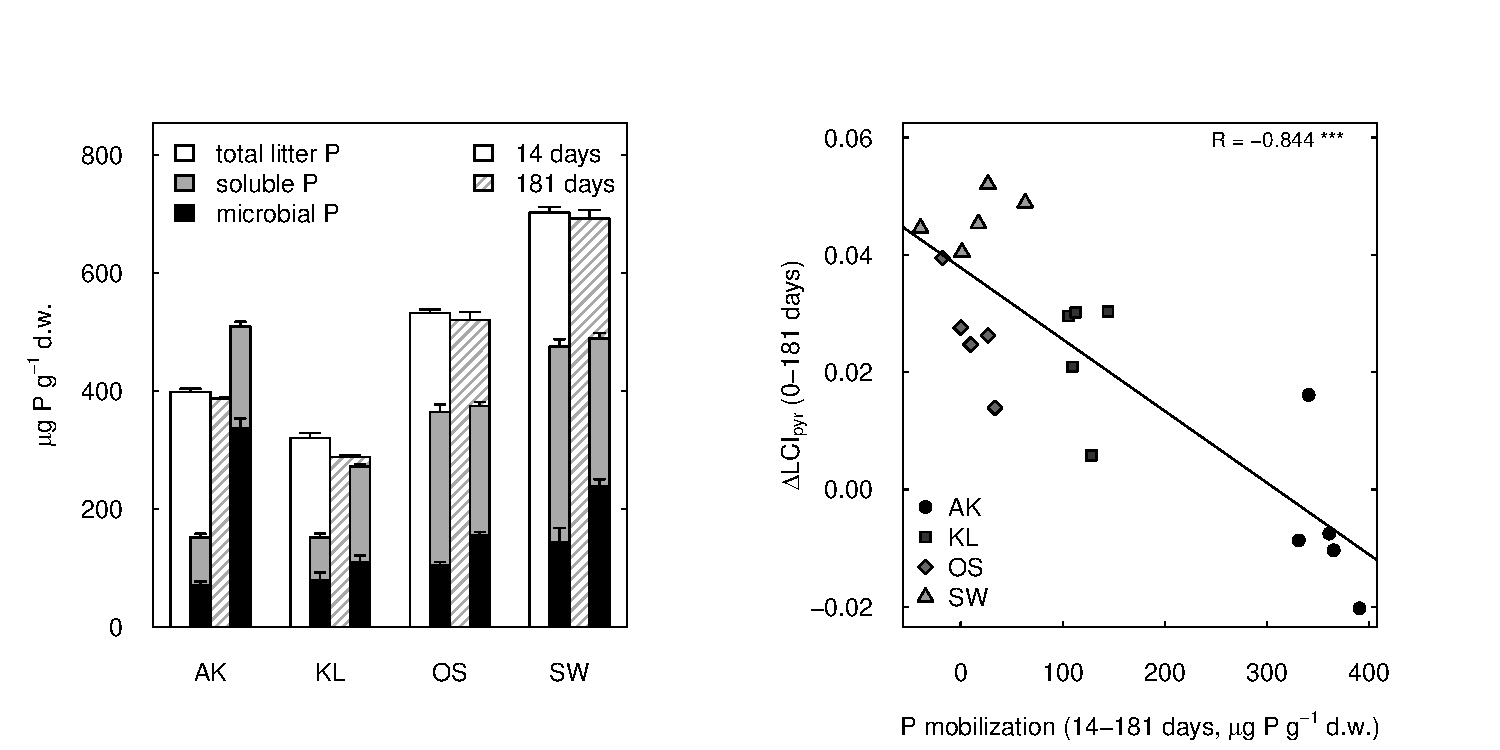
\includegraphics{ligpaper-figphos}
\end{center}
\caption{
{\bf Mobilization of litter P} Left: In lignin degrading litter (AK and KL) a net mobilization of Insoluble litter P into the fast turn-over P pools (soluble P and microbial biomass P) occured over the first 6 months incubation. In non lignin-degrading litter (OS and SW) increases biomass P corresponded with decreases in soluble P, i.e., no additional insoluble P mobilized. Right: correlation between P mobilization and lignin accumulation, 0-6 months incubation. Beech litter was collected in: Schottenwald (SW), triangles; Ossiach (OS), diamonds; Klausenleopoldsdorf (KL), squares; Achenkirch (AK), circles. Error bars indicate standard errors (n=5).}
%\label{fig:phos}
\end{figure}

\begin{figure}[!h]
\begin{center}
%\setkeys{Gin}{width=4in}
%\setkeys{Gin}{width=\textwidth}
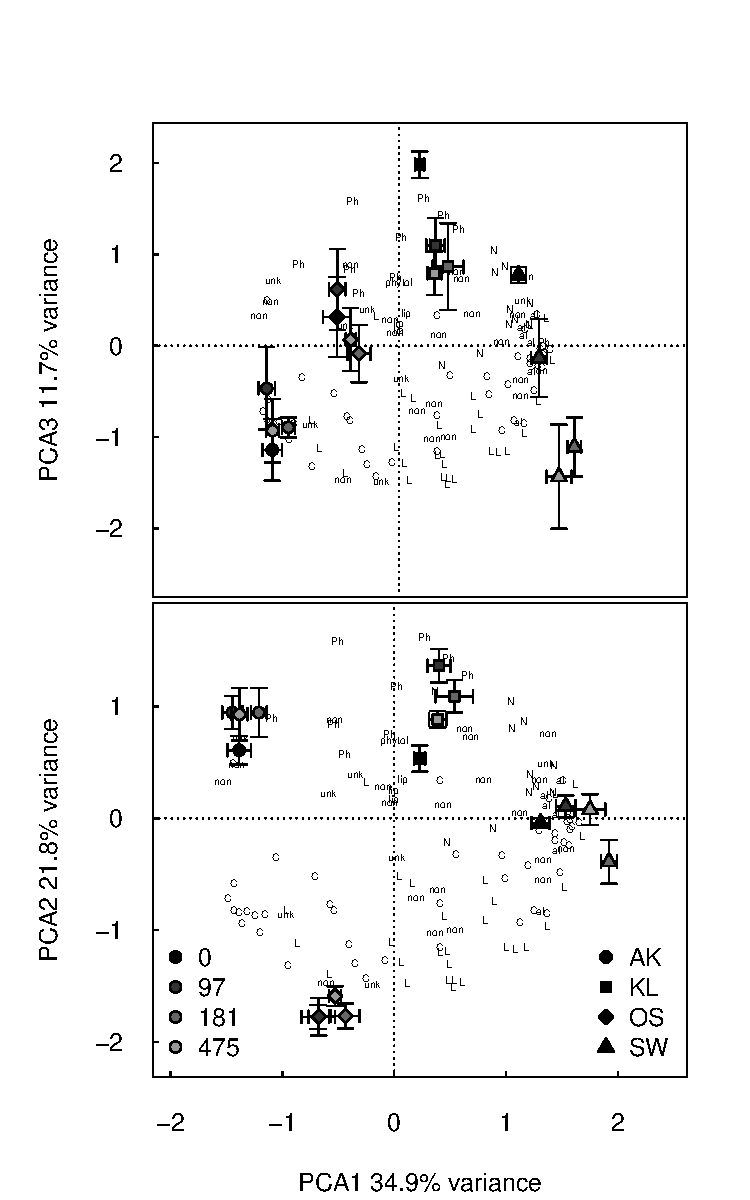
\includegraphics{ligpaper-prypca}
\end{center}
\caption{
{\bf caption} caption.}
%\label{fig:pyrpca}
\end{figure}


\end{document}


